\h{Biological and Psychological Implications}

\begin{refsection}[references/0001_4_bio_psycho_impl.bib]

\section{Regional Contributions to Consciousness}

The differential contribution of brain regions to consciousness reveals fundamental principles about how neural organization supports conscious experience. Perhaps the most striking example emerges from the cerebellum, which despite containing roughly eighty percent of the brain's neurons, appears to make no direct contribution to consciousness \cite{Herculano-Houzel2010}. This remarkable dissociation between neural complexity and conscious processing reveals how consciousness depends on specific patterns of energetic organization rather than mere computational capacity.

The cerebellum's exclusion from consciousness proves particularly instructive when examined through ECC's framework. Despite its sophisticated neural architecture, the cerebellum's highly regular, crystalline circuit organization prevents it from achieving the specific forms of energetic coherence necessary for conscious processing \cite{Ito2008}. Its feedforward processing architecture, limited internal feedback loops, and absence of recursive organization create patterns of neural activity that, while computationally powerful, fail to support conscious experience. This distinctive architecture reveals crucial requirements for consciousness that extend beyond simple information processing.

Cortical regions, by contrast, demonstrate architectural features that specifically support conscious processing \cite{Fox2005}. Their dense reciprocal connectivity, multiple feedback pathways, and complex laminar organization create conditions necessary for maintaining coherent conscious states. The diverse cell types and rich oscillatory dynamics of cortical circuits enable flexible patterns of energetic coherence that can support conscious experience. This architectural contrast between cerebellum and cortex illuminates how consciousness emerges from specific forms of neural organization.

The organization of energy dynamics reveals further distinctions between conscious and unconscious processing regions \cite{Dehaene2006}. The cerebellum maintains highly efficient but stereotyped patterns of energy flow, with limited internal gradients and rigid information pathways. Cortical regions, however, demonstrate complex energy landscapes with multiple stable states and flexible distribution patterns. This difference in energetic organization helps explain why certain neural architectures support consciousness while others, despite their complexity, do not.

Astrocytic networks show particularly significant regional variations that influence conscious processing \cite{Buckner2008}. The cerebellum's specialized Bergmann glia differ markedly from cortical astrocytes in their network organization and calcium signaling properties. These differences in glial architecture shape how regions maintain coherent states and distribute energy, proving crucial for determining their contribution to conscious experience. The resulting patterns of cellular interaction help establish whether regions can support conscious processing.

The thalamus demonstrates another crucial pattern of regional specialization in conscious processing \cite{Balleine2010}. Its unique architecture, combining focused relay nuclei with broader modulatory systems, creates conditions necessary for integrating information into conscious experience. The precise organization of thalamocortical circuits enables both selective attention and broader awareness, while maintaining specific patterns of energetic coherence.

The distinction between primary sensory areas and association cortices reveals additional principles about regional contributions to consciousness \cite{Shulman1997}. Primary areas maintain precise topographic organizations that support detailed sensory processing, while association areas demonstrate more flexible architectures that enable complex integration. These different organizational patterns reflect distinct strategies for maintaining coherent states while supporting different aspects of conscious experience \cite{Allen2016}. The resulting hierarchy of processing reveals how consciousness emerges from coordinated activity across specialized regions.

Subcortical structures present varying degrees of contribution to consciousness that reflect their specific architectural properties \cite{Lou2004}. The brainstem's reticular activating system proves essential for maintaining conscious states through its broad modulatory influences, while basal ganglia circuits shape the content of consciousness through selective gating of information \cite{Parvizi2001}. These different contributions emerge from distinct patterns of cellular organization and energy management that support specific aspects of conscious processing.

The hippocampus presents a particularly interesting case in consciousness, as it proves crucial for conscious memory while operating through distinct computational principles from neocortex \cite{Vogt2005}. Its unique architecture, combining highly organized cellular layers with extensive recurrent connectivity, enables both precise encoding of experiences and their integration into conscious memory. This specialized organization demonstrates how different neural architectures can support distinct aspects of conscious processing through specific patterns of energetic coherence.

Regional variations in neurotransmitter systems add another layer to understanding consciousness \cite{Tononi2016}. Different areas maintain distinct combinations of neurotransmitter receptors and modulatory inputs that shape their contribution to conscious processing. These molecular specializations enable regions to participate in conscious experience in specific ways while maintaining appropriate patterns of energetic coherence. The resulting chemical diversity helps establish the rich landscape of possible conscious states.

The evolution of regional specialization reveals deeper principles about how consciousness emerges from neural organization \cite{Yu2015}. The precise patterns of cellular architecture, connectivity, and molecular specialization that support consciousness appear to have developed through careful refinement of energetic coherence rather than simply increasing computational power. This evolutionary perspective helps explain both why consciousness requires specific neural architectures and how these structures emerged through natural selection.

The functional integration of specialized regions demonstrates sophisticated principles of conscious organization \cite{Schmahmann2019}. Different areas must maintain their unique processing capabilities while participating in broader patterns of conscious integration. This balance between specialization and unity emerges from specific patterns of energetic coherence that enable both local processing and global coordination.

Perhaps most significantly, understanding regional contributions through ECC's framework reveals fundamental principles about the nature of consciousness itself \cite{Vogt2005}. Rather than emerging from computation alone, consciousness requires specific forms of energetic organization that can only be achieved through particular neural architectures. This understanding proves essential for both theoretical developments in consciousness studies and practical applications in treating neurological disorders.

The implications extend beyond neuroscience to broader questions about consciousness in biological and artificial systems \cite{Tononi2016}. The specific requirements for conscious processing revealed through regional specialization suggest why consciousness cannot emerge from arbitrary neural organization, regardless of computational sophistication. This perspective challenges purely computational approaches to consciousness while suggesting new directions for developing artificial systems capable of supporting conscious-like processing.

Regional variations in conscious processing become particularly evident during transitions between wake and sleep states \cite{Dehaene2006}. Different brain regions demonstrate distinct patterns of deactivation and reactivation during sleep onset, revealing fundamental principles about how consciousness depends on coordinated activity across specialized neural architectures \cite{Fox2005}. These regional differences in sleep-wake transitions provide a natural bridge to examining how the brain maintains and modifies conscious states through sophisticated management of energy dynamics during sleep.

Moving from regional organization to state transitions, we must now examine how the brain coordinates changes in consciousness during sleep. Unlike death, where energy gradients collapse entirely, or anesthesia, where they become deliberately disrupted, sleep represents a coordinated reorganization of neural energetics that preserves the capacity for conscious processing while enabling essential restoration and maintenance.

\section{Sleep States and Energy Dynamics}

The transition between wakefulness and sleep reveals fundamental principles about how consciousness depends on specific patterns of energetic organization. During sleep, the brain undergoes profound changes in its physical and energetic architecture, particularly in the management of extracellular space and fluid dynamics \cite{Xie2013}. Unlike death, where energy gradients collapse entirely, or anesthesia, where they become deliberately disrupted, sleep represents a coordinated reorganization of neural energetics that maintains the capacity for conscious processing while enabling essential restoration and maintenance.

During sleep states, the brain's extracellular space expands dramatically, increasing by up to sixty percent compared to wakefulness \cite{Nedergaard2020}. This physical reorganization enables enhanced flow of cerebrospinal fluid through neural tissues, creating conditions necessary for clearing metabolic waste products that accumulate during conscious processing. Astrocytic networks coordinate remarkable volume changes that facilitate this enhanced fluid movement while maintaining overall tissue integrity. These coordinated changes in physical organization demonstrate how consciousness requires specific arrangements of neural space that must be periodically reconfigured.

Brain wave patterns undergo systematic reorganization during sleep transitions, revealing how conscious processing depends on particular patterns of energetic coherence \cite{Scammell2017}. The shift from wake to sleep involves carefully orchestrated changes in oscillatory activity across multiple frequency bands. These altered rhythms reflect fundamental changes in how neural circuits maintain coherent states, demonstrating that consciousness requires specific patterns of energetic organization rather than mere neural activity. The precise regulation of these transitions reveals sophisticated mechanisms for maintaining neural function while enabling necessary periods of reorganization.

The regulation of ion concentrations and metabolic gradients during sleep demonstrates another crucial aspect of consciousness's energetic requirements \cite{DiNuzzo2017}. Neural tissues maintain careful control over ion distributions and energy availability even during sleep, though in distinctly different patterns from wakefulness. This preservation of basic energetic organization, despite profound changes in neural activity, explains why consciousness can readily return upon awakening. The contrast with death, where these gradients collapse irreversibly, reveals how consciousness depends on maintaining specific patterns of energetic coherence.

The glymphatic system becomes particularly active during sleep, enabling enhanced exchange between cerebrospinal fluid and interstitial fluid throughout neural tissues \cite{Nedergaard2020}. This increased fluid movement supports crucial processes of cellular repair and waste clearance while requiring specific patterns of tissue organization distinct from wakefulness. The coordination between fluid dynamics and neural activity during sleep reveals sophisticated mechanisms for maintaining brain function while enabling necessary maintenance processes.

The molecular and cellular mechanisms underlying sleep transitions demonstrate remarkable sophistication in managing neural energetics \cite{Holst2018}. Ion pumps adjust their activity to maintain essential gradients while operating at reduced levels, metabolic processes shift to support repair and restoration, and neural circuits modify their firing patterns to enable sustained periods of reduced activity. These coordinated changes in cellular function reveal how consciousness requires precise management of energy dynamics across multiple scales of organization.

The role of astrocytic networks becomes particularly significant during sleep states \cite{Krueger2016}. These glial cells coordinate volume changes that enable enhanced fluid flow through neural tissues while maintaining essential ionic balance and metabolic support. Their ability to regulate both cellular energetics and extracellular space properties proves crucial for enabling the brain to transition between conscious states while preserving fundamental organization. The resulting patterns of glial activity demonstrate how consciousness emerges from coordinated cellular interactions rather than neuronal activity alone.

Sleep's impact on synaptic organization reveals another crucial aspect of consciousness's energetic requirements \cite{Cirelli2015}. During sleep, synaptic strengths undergo systematic modification, generally trending toward reduction in what has been termed synaptic homeostasis. This process enables more efficient energy utilization while preserving essential information encoded in synaptic patterns. The careful regulation of synaptic reorganization during sleep demonstrates how consciousness requires ongoing management of energy investments in neural connectivity.

The relationship between sleep and memory consolidation highlights sophisticated mechanisms for maintaining information while reorganizing energy dynamics \cite{Rasch2013}. During sleep, the brain can strengthen important synaptic connections while weakening others, creating more efficient patterns of connectivity that support both energy conservation and information preservation. This process reveals how consciousness depends on careful balance between stability and plasticity in neural organization.

The circulation of cerebrospinal fluid during sleep demonstrates particularly elegant mechanisms for maintaining neural function \cite{Xie2013}. Enhanced flow through the recently discovered glymphatic system enables efficient clearing of metabolic waste products while delivering essential nutrients to neural tissues. This coordinated movement of fluid through expanding extracellular spaces reveals how consciousness requires sophisticated management of the brain's physical environment.

The coordination between these various physiological changes during sleep reveals deeper principles about consciousness itself \cite{Saper2017}. Rather than representing a simple shutdown of conscious processing, sleep emerges as a sophisticated state of altered coherence that enables essential maintenance while preserving the capacity for rapid return to consciousness. This carefully managed transition between states demonstrates how consciousness depends on specific patterns of energetic organization that can be temporarily modified without being fundamentally disrupted.

Sleep-dependent modulation of neural circuits reveals sophisticated principles of energy management \cite{Vyazovskiy2013}. Different brain regions undergo coordinated but distinct patterns of activity modification, enabling both local restoration and maintenance of global organization. This regional variation in sleep-related changes demonstrates how consciousness emerges from the precise orchestration of multiple parallel processes.

Perhaps most significantly, the study of sleep through ECC's framework reveals how consciousness requires continuous management of energy dynamics across multiple scales of organization \cite{Scammell2017}. The brain's ability to maintain essential coherence while dramatically altering its operating mode demonstrates that consciousness emerges from specific patterns of energetic organization rather than mere neural activity. This understanding suggests new approaches to both studying consciousness and treating disorders that affect sleep-wake transitions.

The role of neuromodulatory systems in sleep regulation demonstrates sophisticated control over brain state transitions \cite{Zhang2018}. Different neurotransmitter systems coordinate their activity to enable smooth transitions between wake and sleep states while maintaining the brain's essential organizational principles. This chemical orchestration reveals fundamental mechanisms for modifying conscious states while preserving the capacity for consciousness itself.

The implications extend beyond neuroscience to fundamental questions about the nature of consciousness itself \cite{Krueger2016}. The remarkable sophistication of sleep regulation demonstrates how biological systems achieve conscious processing through careful management of energy dynamics rather than abstract computation. This perspective challenges purely computational approaches to consciousness while suggesting new directions for developing artificial systems capable of supporting conscious-like processing.

Moving from normal sleep-wake transitions to pathological conditions, we must now examine how disruptions of energy dynamics can alter or eliminate conscious processing \cite{Mander2017}. These disorders - ranging from minimally conscious states to persistent vegetative states - reveal how different patterns of energetic disruption lead to distinct impairments of consciousness while sometimes maintaining basic biological viability.

\section{Disorders of Consciousness}

The study of consciousness disorders provides crucial insights into how disruptions of energy dynamics can alter or impair conscious experience while sometimes maintaining basic biological viability. These conditions, ranging from minimally conscious states to persistent vegetative states, reveal how different patterns of energetic disruption lead to distinct impairments of consciousness \cite{Giacino2014}. Through careful examination of these disorders, we gain fundamental understanding of how consciousness emerges from and requires specific patterns of energetic coherence.

In the vegetative state, the brain maintains basic biological functions but shows profound disruption of the energy dynamics necessary for conscious experience \cite{Laureys2004}. This condition demonstrates particularly striking dissociation between biological viability and consciousness, as patients maintain essential autonomic functions while showing severe impairment of the energetic patterns that support conscious processing. The disruption of neural synchronization, altered metabolic coupling between neurons and glia, and impaired long-range information integration reveal how consciousness requires specific forms of energetic coherence beyond mere biological survival.

Minimally conscious states present a different pattern of energetic disruption, characterized by fluctuating periods of awareness and responsiveness \cite{DiPerri2014}. These conditions demonstrate how consciousness can persist in fragmentary form when some patterns of energetic coherence remain partially intact. The intermittent nature of conscious awareness in these cases reveals how consciousness requires sustained patterns of coherent energy flow rather than merely achieving threshold levels of neural activity. The variable maintenance of conscious processing in these states provides unique insights into the minimal requirements for conscious experience.

Locked-in syndrome represents another crucial variant that illuminates fundamental principles about consciousness \cite{Casali2013}. In this condition, consciousness remains largely preserved despite severe disruption of motor output pathways. The maintenance of coherent energy dynamics within cognitive networks, despite profound impairment of motor systems, demonstrates how consciousness can persist when core patterns of energetic coherence remain intact. This selective preservation of conscious processing reveals important distinctions between the neural mechanisms supporting consciousness itself and those enabling behavioral output.

Coma presents perhaps the most severe disruption of consciousness, characterized by global depression of brain activity and severely reduced energy consumption \cite{Adams2000}. The profound alterations in neurotransmitter systems, disrupted extracellular space regulation, and impaired astrocytic network function in coma demonstrate how consciousness requires coordinated energy dynamics across multiple cellular systems. The potential for recovery from coma, unlike brain death, suggests that some fundamental organization remains preserved even in this deeply unconscious state.

These distinct disorders reveal crucial aspects about the organization of consciousness through their different patterns of disruption and preservation \cite{Monti2010}. Hemispheric neglect, for instance, demonstrates how consciousness can maintain coherence even with significant localized disruption. The preservation of consciousness with altered content, rather than global impairment, suggests that conscious processing possesses modular aspects while requiring broader integration.

Drawing on recent empirical work detailed in \cite{LeVanQuyen2007} and \cite{Bartolomei2009}, we can understand how excessive neural synchronization can paradoxically lead to loss of consciousness, demonstrating that synchrony alone is insufficient for conscious experience. This reveals a crucial distinction between mere neural synchronization and the meaningful integration of information required for consciousness \cite{Koch2016,Tononi2015}.

Studies of epileptic seizures provide compelling evidence for this principle. During seizure events, neural populations exhibit extreme synchronization, yet this often results in loss of consciousness rather than enhanced awareness \cite{Bartolomei2009}. The key insight is that consciousness requires not just coordinated neural firing, but specific patterns of functional integration that maintain distinct information across neural populations while enabling meaningful interaction between them.

When neural synchrony becomes excessive, as in seizure states, it can actually disrupt the delicate balance of integration and differentiation necessary for conscious processing. Research has shown that seizure-induced unconsciousness correlates with increased long-distance synchronization between cortical and subcortical structures \cite{Bartolomei2009}. This suggests that too much synchronization can paradoxically reduce the brain's capacity for information integration by collapsing normally distinct neural populations into a single undifferentiated pattern of activity.

Furthermore, studies examining pre-seizure states demonstrate that consciousness requires specific patterns of coordinated activity rather than synchronization per se \cite{LeVanQuyen2002}. The transition from normal consciousness to seizure-induced unconsciousness involves distinct changes in how neural populations interact, with excessive synchronization actually disrupting the precise temporal relationships that support conscious integration.

This understanding aligns with broader theoretical work on consciousness which emphasizes that conscious experience emerges from the brain's capacity to balance differentiation and integration of information \cite{Koch2016}. When neural synchrony becomes too strong or too widespread, it can disrupt this balance by reducing the brain's ability to maintain distinct patterns of information while still enabling meaningful interaction between different neural populations.

The implications extend beyond epilepsy to other disorders of consciousness. By recognizing that consciousness requires specific patterns of functional integration rather than mere synchronization, we gain deeper insight into how various pathological conditions might disrupt conscious experience through different mechanisms of neural dysregulation. This suggests new approaches to treating disorders of consciousness by focusing on restoring appropriate patterns of functional integration rather than simply modulating neural synchrony.

The role of astrocytic networks proves particularly significant in this context \cite{Tononi2015}. These networks help maintain appropriate patterns of neural integration through sophisticated regulation of local circuit activity. When this regulation fails, as in seizure states, the resulting pattern of excessive synchronization can paradoxically reduce rather than enhance conscious integration. This demonstrates how consciousness emerges from carefully regulated patterns of neural interaction rather than simple synchronization.

Brain death represents the terminal case of consciousness disruption, marked by complete loss of organized energy dynamics and irreversible breakdown of cellular gradients \cite{Wijdicks2010}. Unlike other disorders where some patterns of coherence persist, brain death involves collapse of all integration capacity and permanent disruption of the conscious substrate. This ultimate loss of consciousness demonstrates how the physical basis of conscious experience depends on maintaining specific patterns of energetic organization that, once lost, cannot be restored.

The hierarchical nature of consciousness becomes particularly evident through these disorders \cite{Baars2005}. Basic biological functions can persist without consciousness, while different levels of conscious processing can be separately impaired. This stratification reveals how consciousness emerges from increasingly sophisticated patterns of energetic coherence built upon more fundamental biological processes. The selective impairment or preservation of different aspects of consciousness demonstrates how specific patterns of coherence support distinct features of conscious experience.

Recovery patterns from disorders of consciousness provide additional insights into the nature of conscious processing \cite{Schiff2010}. Different trajectories of recovery, based on the type of energetic disruption, suggest that consciousness requires specific forms of coherence that must be restored in particular sequences. The importance of reestablishing proper patterns of energy flow proves crucial for recovery, while the critical periods for intervention reveal temporal constraints on maintaining conscious organization.

The relationship between metabolic activity and consciousness becomes particularly clear through these disorders \cite{Massimini2005}. While some brain regions may maintain metabolic activity without contributing to consciousness, conscious processing appears to require specific patterns of energetic coherence rather than merely achieving threshold levels of metabolism. This distinction helps explain why certain patterns of brain activity fail to support consciousness despite maintaining basic cellular function.

The therapeutic implications of understanding consciousness disorders through ECC's framework suggest new approaches to treatment and rehabilitation \cite{Giacino2014}. Rather than focusing solely on restoring neural activity, interventions might target the reestablishment of specific patterns of energetic coherence. This perspective suggests why certain therapeutic approaches prove more effective than others, while indicating new directions for developing treatments that specifically address the disrupted patterns of energy organization underlying different disorders of consciousness.

The role of network connectivity in consciousness disorders reveals sophisticated principles of neural organization \cite{Dehaene2011}. Different patterns of network disruption lead to distinct impairments in conscious processing, suggesting that consciousness emerges from specific configurations of energetic coherence across neural networks. This understanding helps guide both diagnostic approaches and therapeutic interventions.

Perhaps most significantly, the study of consciousness disorders through ECC's framework reveals fundamental principles about how consciousness emerges from biological organization \cite{Tononi2015}. Rather than representing simple loss of neural activity, these conditions demonstrate how consciousness requires specific patterns of energetic coherence that can be disrupted in distinct ways. This understanding proves essential for both theoretical developments in consciousness studies and practical approaches to treating disorders of consciousness.

The implications extend beyond clinical practice to fundamental questions about the nature of consciousness itself \cite{Laureys2004}. The various ways consciousness can be disrupted while maintaining biological viability demonstrate that consciousness emerges from specific patterns of energetic organization rather than mere neural activity. This perspective challenges purely computational approaches to consciousness while suggesting new directions for both scientific investigation and therapeutic intervention.

The differential contribution of brain regions to consciousness represents one of the most striking features of neural organization \cite{Baars2005}. While regions like the cortex and thalamus prove crucial for conscious experience, others like the cerebellum - despite containing roughly eighty percent of the brain's neurons - appear to make no direct contribution to consciousness. This distinction reflects fundamental differences in how these regions organize and process energy \cite{DiPerri2014}.

Moving from disorders of consciousness to altered states, we must now examine how anesthesia deliberately and reversibly disrupts the specific mechanisms required for conscious processing. Unlike sleep or coma, anesthetic agents create precisely controlled perturbations that reveal fundamental principles about how consciousness emerges from and requires specific patterns of energetic coherence.

\section{Anesthesia and Consciousness}

General anesthesia represents a unique state where consciousness is deliberately and reversibly abolished through specific disruption of energy dynamics. Unlike sleep, where basic patterns of energetic organization are preserved, or death, where energy gradients collapse entirely, anesthesia creates a controlled disruption of the mechanisms required for conscious processing \cite{Alkire2008}. This precise intervention in neural function provides crucial insights into how consciousness emerges from and requires specific patterns of energetic coherence.

The primary mechanisms through which anesthetic agents abolish consciousness reveal fundamental principles about conscious processing \cite{Franks2008}. Through disruption of membrane protein function, alteration of ion channel dynamics, and modification of synaptic transmission, these compounds specifically target the physical substrates that support conscious states. Unlike crude suppression of neural activity, anesthetics create sophisticated patterns of disruption that specifically abolish consciousness while maintaining essential biological functions.

The energy dynamic changes induced by anesthesia demonstrate remarkable specificity in their effects \cite{Brown2010}. While disrupting the patterns of coherence necessary for consciousness, anesthetic agents maintain cellular viability and preserve basic energy gradients. This selective action enables both the reliable elimination of consciousness and its subsequent restoration when the drugs are cleared. The resulting state differs fundamentally from both sleep and coma, representing a precisely controlled disruption of conscious processing.

The molecular mechanisms of general anesthetics provide particular insight into consciousness \cite{John2005}. Different classes of anesthetic agents, despite varying molecular targets, ultimately converge on disrupting the specific patterns of neural coherence required for conscious experience. The common end result of unconsciousness, achieved through diverse molecular pathways, reveals fundamental principles about how consciousness emerges from neural organization.

The relationship between anesthetic depth and consciousness reveals sophisticated principles of neural organization \cite{Sanders2012}. As anesthetic concentrations increase, consciousness dissolves through predictable stages that reflect progressive disruption of coherent processing. This gradual degradation of conscious experience demonstrates how consciousness requires specific patterns of energetic organization that can be systematically disrupted while maintaining basic neural function.

The pharmacological mechanisms of different anesthetic agents reveal distinct pathways to disrupting conscious processing \cite{Uhrig2018}. The variety of molecular targets through which different anesthetics achieve unconsciousness, while still maintaining vital functions, demonstrates the specific requirements for conscious processing. This pharmacological dissection of consciousness provides unique insights into its fundamental mechanisms.

\begin{figure}[h]
    \centering
    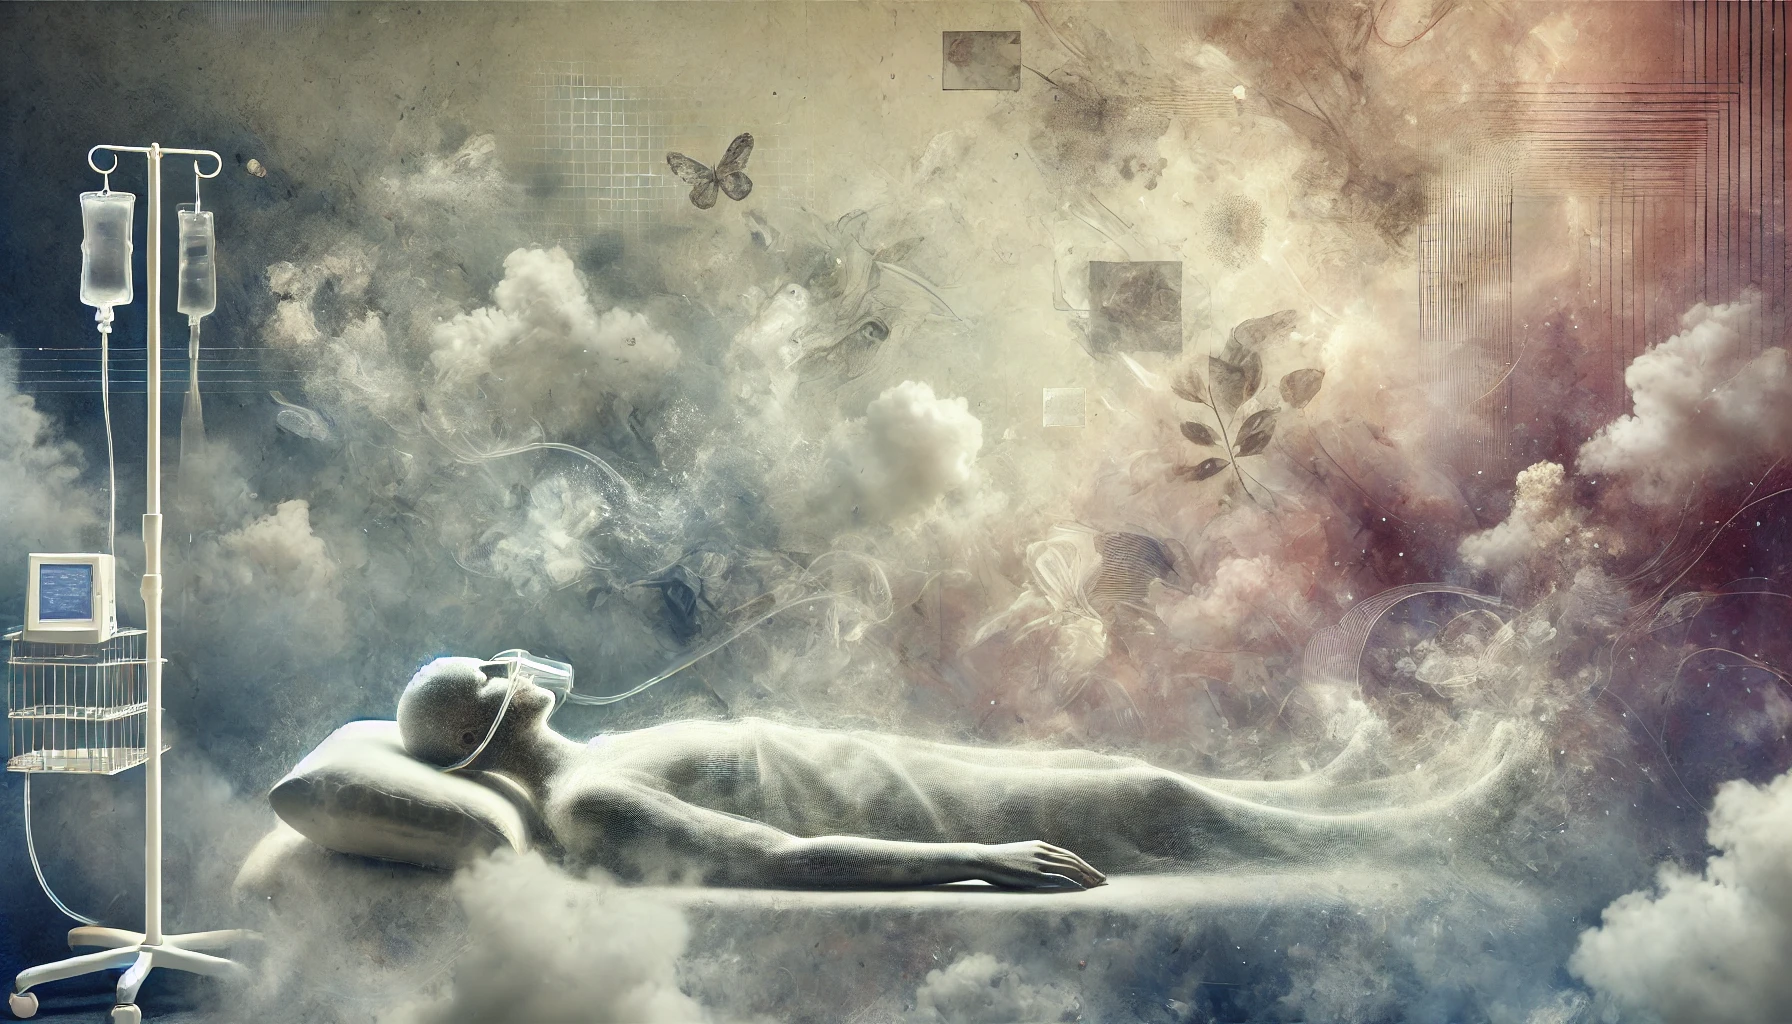
\includegraphics[width=0.8\textwidth]{anesthesia.png}

    \caption{Artistic depiction of a person under anesthesia. }
\end{figure}

The spatial organization of anesthetic effects proves particularly revealing about consciousness \cite{Lewis2012}. Rather than producing uniform suppression across neural tissues, anesthetics create specific patterns of disruption that target the networks and connections crucial for conscious processing. This anatomical specificity helps explain why consciousness can be eliminated while preserving essential physiological functions. The resulting patterns of neural activity demonstrate how consciousness requires particular forms of network organization beyond mere neural activation.

The temporal dynamics of anesthetic action provide additional insights into conscious processing \cite{Purdon2013}. The transition into unconsciousness often occurs more rapidly than emergence, revealing fundamental asymmetries in how consciousness is maintained and restored. These temporal patterns suggest that consciousness requires specific sequences of energetic organization that can be quickly disrupted but need more coordinated processes for re-establishment. The precise timing of these transitions helps illuminate the dynamic requirements for conscious processing.

The preservation of certain neural functions under anesthesia while eliminating consciousness reveals crucial distinctions in neural processing \cite{Sanders2012}. Many basic reflexes and autonomic functions continue during anesthesia, demonstrating that sophisticated neural activity can persist without supporting conscious experience. This dissociation helps identify the specific patterns of energetic coherence that consciousness requires, distinct from other forms of neural processing.

The interaction between anesthetic agents and brain rhythms reveals fundamental principles about conscious organization \cite{Steriade2003}. Different anesthetics produce characteristic changes in oscillatory patterns that correlate with the loss and recovery of consciousness. These effects suggest that proper orchestration of brain rhythms proves essential for conscious processing, while specific disruptions of these rhythmic patterns can systematically eliminate consciousness while preserving basic neural function.

The role of thalamocortical circuits in anesthetic-induced unconsciousness demonstrates key principles about conscious processing \cite{Mashour2017}. Anesthetics specifically disrupt the patterns of communication between thalamus and cortex that support conscious integration. This targeted effect on thalamocortical coherence reveals fundamental mechanisms necessary for maintaining conscious states.

The differential sensitivity of neural circuits to anesthetics provides insights into consciousness \cite{Tonner2017}. Certain neural pathways prove particularly vulnerable to anesthetic disruption, while others maintain function even at deep levels of anesthesia. This selective effect helps identify the specific circuits and mechanisms most crucial for conscious processing.

The implications of anesthetic mechanisms extend beyond clinical practice to fundamental questions about consciousness itself \cite{Alkire2008}. The ability to precisely and reversibly eliminate consciousness through specific molecular interventions demonstrates that consciousness requires particular patterns of energetic organization rather than emerging from computation alone. This understanding suggests new approaches to both studying consciousness and developing more sophisticated methods for controlling conscious states.

Perhaps most significantly, anesthesia reveals how consciousness depends on specific physical mechanisms that can be systematically disrupted \cite{Brown2010}. Unlike philosophical thought experiments about consciousness, anesthesia provides concrete evidence for the physical basis of conscious experience through reliable and reversible manipulation of conscious states. This empirical grounding proves essential for developing both theoretical understanding of consciousness and practical applications in medicine.

The study of anesthesia through ECC's framework suggests new directions for research and clinical practice \cite{Franks2008}. Rather than focusing solely on receptor binding or neural activity patterns, this perspective emphasizes how different anesthetic agents converge on disrupting specific patterns of energetic coherence necessary for consciousness. This understanding could lead to more precisely targeted anesthetic agents and better methods for monitoring depth of anesthesia.

Unlike anesthetics, which suppress consciousness, psychedelics and other psychoactive compounds modify conscious experience by altering patterns of energy flow and neural synchronization while maintaining basic coherence \cite{John2005}. These substances create distinctive alterations in consciousness through specific modulation of neural dynamics. Moving forward, we must examine how these compounds reshape conscious experience through targeted changes in brain organization and energy flow.

\section{Altered States of Consciousness}

The study of altered states reveals fundamental principles about conscious processing through examining how various compounds can profoundly modify experience while maintaining basic coherence. Unlike anesthetics, which suppress consciousness entirely, psychedelics and other psychoactive substances reshape conscious experience through specific modulation of neural dynamics and energy flows \cite{CarhartHarris2019}. These chemical interventions demonstrate how consciousness can maintain coherent organization while undergoing dramatic alterations in its qualitative character.

Classical psychedelics like LSD and psilocybin create particularly striking modifications of conscious experience through their effects on serotonin systems \cite{Nichols2016}. By activating 5-HT2A receptors, these compounds enhance neural plasticity and fundamentally alter patterns of brain synchronization. The resulting changes in default mode network activity and information integration reveal how consciousness can maintain coherent processing while operating in radically different modes. These substances demonstrate how specific molecular interventions can reliably induce profound but organized changes in conscious experience.

The role of set and setting in psychedelic experiences reveals sophisticated principles of conscious regulation \cite{Zinberg1984}. The same compounds can produce markedly different effects depending on psychological and environmental context, demonstrating how consciousness integrates multiple levels of influence in creating coherent experience. This context-dependency shows how altered states emerge from the interaction between specific molecular mechanisms and broader patterns of neural organization.

Network analysis reveals how different classes of psychoactive compounds create distinct patterns of alteration in conscious processing \cite{Preller2018}. Psychedelics tend to increase global connectivity while disrupting normal hierarchical processing, enabling enhanced cross-modal integration and novel patterns of association. These different patterns of network reorganization demonstrate how consciousness can maintain coherent function while operating through dramatically altered configurations.

The relationship between altered states and energy metabolism reveals sophisticated principles of conscious organization \cite{Vaitl2005}. Psychedelics and stimulants create distinct patterns of metabolic demand, adjusting how neural circuits utilize and distribute energy. These changes in metabolic dynamics demonstrate how consciousness can sustain coherent processing through different energetic regimes. The precise coordination between altered neural activity and energy metabolism proves essential for maintaining conscious states during these profound modifications.

The temporal dynamics of altered states demonstrate remarkable sophistication in how consciousness maintains coherence through dramatic transitions \cite{Vollenweider2020}. The onset, peak effects, and gradual resolution of psychedelic experiences reveal how conscious processing can undergo profound reorganization while preserving basic stability. These temporal patterns suggest that consciousness possesses intrinsic mechanisms for maintaining coherent function even during radical alterations in its organizing principles.

\begin{figure}[h]
    \centering
    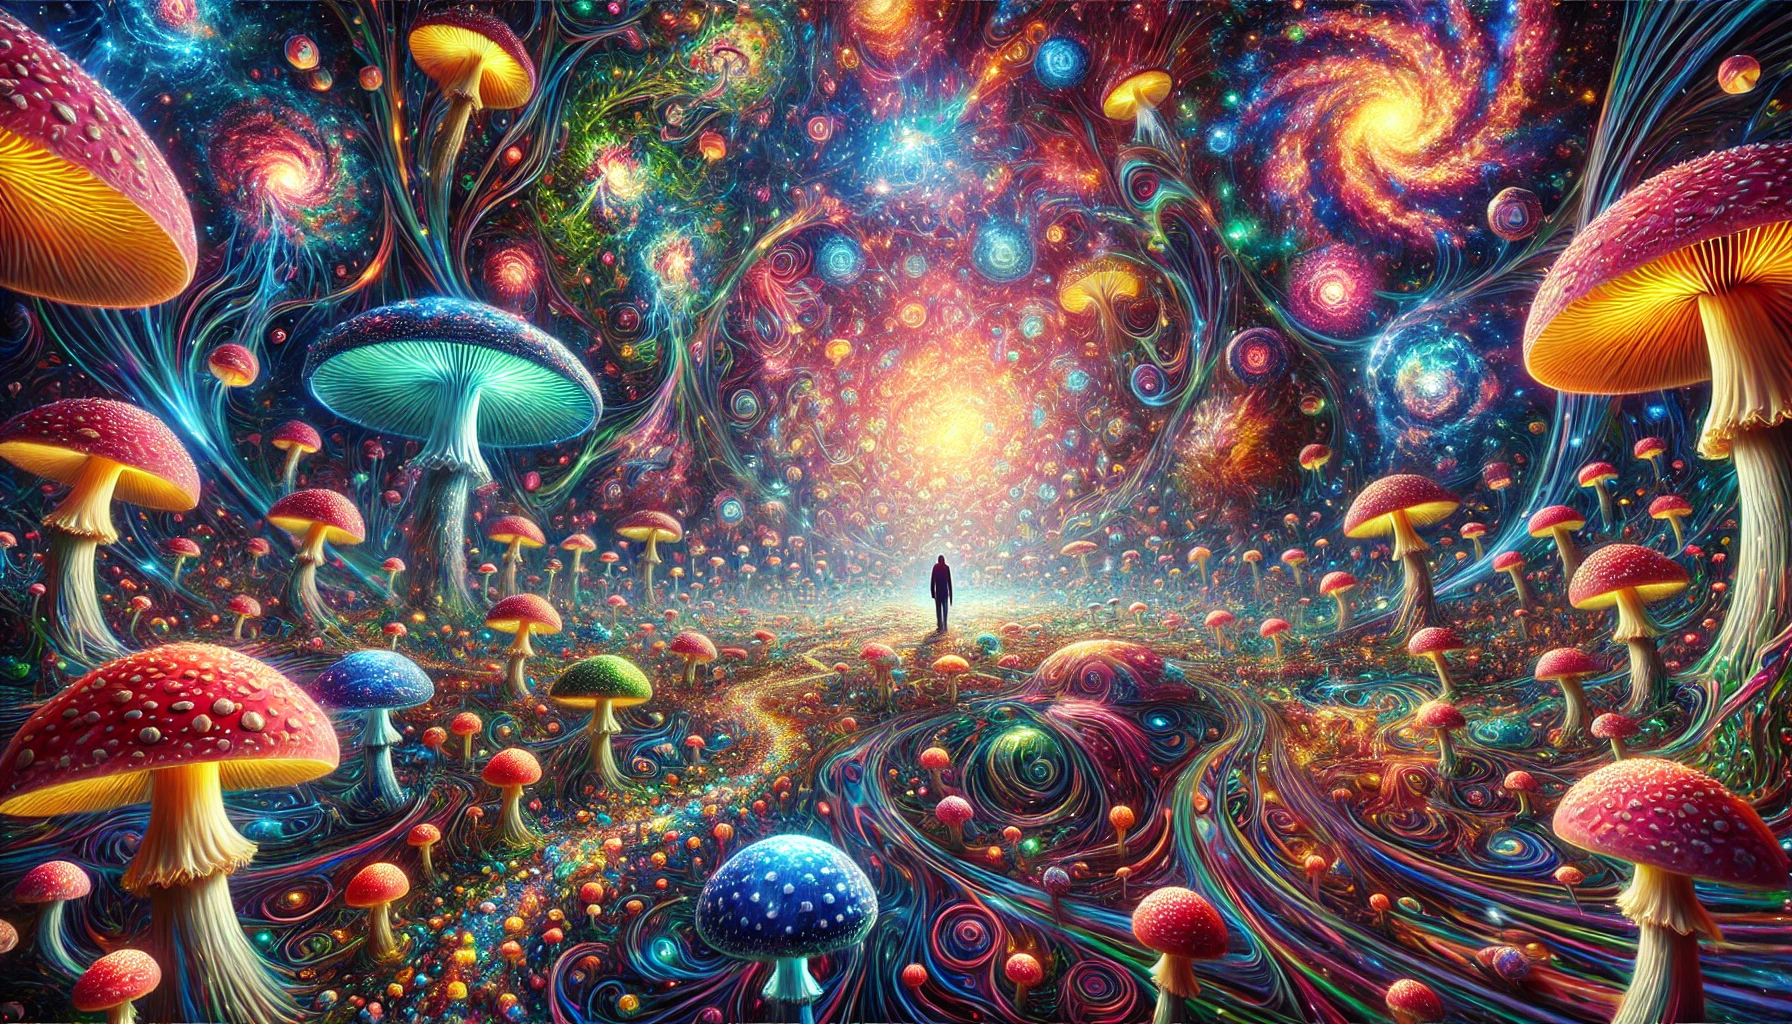
\includegraphics[width=0.8\textwidth]{mushroom_trip.png}

    \caption{A mushroom trip}
\end{figure}

The interaction between different neurotransmitter systems during altered states reveals complex principles of conscious regulation \cite{Ludwig1966}. Psychedelics influence not only serotonin systems but also modulate glutamate release and neural plasticity, creating cascading effects across multiple signaling pathways. These sophisticated patterns of chemical interaction demonstrate how consciousness emerges from coordinated activity across multiple molecular systems rather than single neurotransmitter effects.

Changes in perception during altered states illuminate fundamental aspects of how consciousness constructs experience \cite{Dittrich2010}. The modification of sensory processing, emotional responses, and cognitive associations reveals how consciousness actively organizes information rather than passively receiving it. The maintenance of coherent experience despite dramatic alterations in these organizing principles demonstrates the remarkable flexibility of conscious processing.

The relationship between altered states and the default mode network proves particularly revealing \cite{CarhartHarris2019}. Psychedelics can fundamentally reshape activity in this network while preserving broader conscious function, suggesting that even core aspects of self-experience arise from specific patterns of energetic organization that can be systematically modified. These alterations in self-processing reveal how consciousness maintains coherent experience even when fundamental aspects of cognition become profoundly altered.

Memory formation during altered states demonstrates sophisticated principles of conscious integration \cite{Hobson2007}. Despite profound changes in experience, consciousness maintains the ability to encode and later recall these altered states, suggesting that coherent memory formation can persist even during dramatic reorganization of conscious processing. This preservation of memory function reveals how consciousness maintains essential capabilities even while operating in radically different modes.

The clinical implications of understanding altered states through ECC's framework suggest new therapeutic approaches for various psychological conditions \cite{Vollenweider2020}. The capacity of psychedelics to enable coherent yet profoundly reorganized states of consciousness indicates potential pathways for treating disorders that involve rigid or maladaptive patterns of neural organization. This perspective helps explain both the therapeutic potential of psychedelic compounds and the importance of carefully managed contexts for their administration.

The role of cultural frameworks in shaping altered states reveals important principles about conscious organization \cite{Winkelman2010}. While the underlying neural mechanisms may be similar, the interpretation and expression of psychedelic experiences vary dramatically across cultural contexts. This interaction between biological and cultural factors demonstrates how consciousness integrates multiple levels of organization in creating coherent experience.

Perhaps most significantly, the study of altered states through ECC's framework reveals fundamental principles about the nature of conscious processing \cite{Preller2018}. Rather than representing random disruption of normal function, these states demonstrate how consciousness can maintain coherent organization while operating through radically different patterns of energetic dynamics. This understanding challenges simplified models of consciousness while suggesting new approaches to both scientific investigation and therapeutic application.

The implications extend beyond clinical practice to fundamental questions about the potential range of conscious experience \cite{Wulff2014}. The remarkable variety of altered states achievable through specific molecular interventions suggests that normal waking consciousness represents just one of many possible coherent configurations of neural dynamics. This perspective opens new avenues for understanding both the flexibility and constraints of conscious processing in biological systems.

Unlike pharmacologically induced alterations, trance states and ecstatic experiences represent unique modifications of consciousness that can occur without external intervention \cite{Eliade1964}. These states reveal how internal regulation of energy dynamics can produce profound alterations in conscious experience through sophisticated management of neural coherence \cite{Farthing1992}. Moving forward, we must examine how these endogenous mechanisms reshape conscious experience through voluntary control of brain organization and energy flow.

\section{Trance and Ecstasis}

Trance states and ecstatic experiences reveal unique modifications of consciousness achievable through internal regulation rather than external intervention. Where psychedelics and other compounds alter consciousness through direct molecular action, trance states demonstrate how sophisticated management of neural energetics can produce profound alterations in conscious experience through voluntary control \cite{Rouget1985}. These internally generated modifications of consciousness illuminate fundamental principles about how biological systems can maintain coherent processing while operating in radically altered configurations.

Physiological changes during trance states demonstrate remarkable sophistication in conscious regulation \cite{Becker2004}. Through controlled modulation of breathing patterns, heart rate variability, and autonomic balance, practitioners can systematically alter their conscious experience while maintaining coherent organization. These coordinated physiological changes create specific patterns of brain wave activity that support altered states while preserving essential functional stability. The resulting modifications in consciousness emerge from precise management of biological rhythms rather than random perturbation.

The energy dynamics of trance states reveal particularly sophisticated principles of neural regulation \cite{Lewis2003}. Unlike the broad disruptions caused by pharmacological interventions, trance states involve highly organized patterns of oscillatory activity that maintain specific forms of coherence while enabling profound alterations in experience. These coordinated changes in neural energetics demonstrate how consciousness can achieve dramatic modifications through careful management of intrinsic biological rhythms.

Network reorganization during trance reveals fundamental principles about conscious flexibility \cite{Wier2009}. Reduced activity in the default mode network, enhanced interoceptive processing, and modified sensory gating create distinctive patterns of neural activation that support profound alterations in conscious experience. These changes in network organization demonstrate how internal regulation can reshape conscious processing while maintaining essential coherence. The resulting states enable forms of experience typically inaccessible during normal waking consciousness.

The relationship between trance states and bodily awareness illuminates sophisticated mechanisms of conscious control \cite{Goodman1988}. Through sustained attention to interoceptive signals and careful regulation of physiological processes, practitioners can systematically modify their conscious experience while maintaining organized function. These internally generated alterations demonstrate how consciousness can achieve profound modifications through voluntary regulation rather than external intervention.

The phenomenology of trance states reveals important principles about conscious organization \cite{Lapassade1990}. Practitioners often report experiences of altered self-boundaries, modified temporal perception, and enhanced awareness of subtle bodily processes. These changes in conscious experience emerge from systematic modification of neural dynamics rather than random disruption. The resulting alterations demonstrate how consciousness can maintain coherent function while operating through radically different patterns of self-organization.

\begin{figure}[h]
    \centering
    
\includegraphics[width=0.8\textwidth]{trance.png}

    \caption{A shaman in a state of trance}
\end{figure}

The distinction between different forms of trance illuminates multiple pathways for conscious modification \cite{Bourguignon1973}. Meditative states, shamanic journeying, and possession trance each involve distinct patterns of physiological and neural regulation that produce unique alterations in conscious experience. These various forms of trance reveal how consciousness can achieve profound modifications through different combinations of internal control. The diversity of possible trance states demonstrates the remarkable flexibility of conscious processing.

The role of cultural frameworks in shaping trance experiences proves particularly significant \cite{Lewis2003}. While the underlying neural mechanisms may be similar, the interpretation and expression of trance states vary dramatically across cultural contexts. This interaction between biological and cultural factors demonstrates how consciousness integrates multiple levels of organization in creating coherent experience. The resulting states reflect both universal principles of neural organization and specific cultural patterns of meaning.

The temporal dynamics of trance induction reveal sophisticated principles of conscious regulation \cite{Turner1992}. Rather than sudden shifts in experience, trance states typically develop through graduated stages of physiological and neural reorganization. This progressive modification of conscious processing enables stable transitions between radically different states of awareness. The careful management of these transitions demonstrates how consciousness can maintain coherent function while undergoing fundamental reorganization.

The relationship between trance states and memory formation shows interesting patterns of conscious integration \cite{Jilek1982}. Unlike some drug-induced states, trance experiences often remain accessible to later recall while incorporating elements of both ordinary and extraordinary awareness. This preservation of memory function during profound alterations in consciousness reveals how biological systems can maintain essential capabilities while operating in radically different modes.

The role of trance states in therapeutic contexts reveals promising applications of this understanding \cite{Crapanzano1973}. The capacity for consciousness to achieve profound yet controlled alterations through internal regulation suggests new approaches to treating various psychological conditions. Rather than relying solely on external interventions, therapeutic practices might develop more sophisticated methods for enhancing conscious self-regulation through disciplined practice and cultural scaffolding.

The relationship between trance and social context demonstrates sophisticated principles of conscious modification \cite{Houseman1998}. Many traditional trance practices occur within structured social settings that help guide and stabilize altered states of consciousness. This social scaffolding reveals how conscious regulation can be enhanced through cultural frameworks and interpersonal support.

Perhaps most significantly, the study of trance and ecstatic states through ECC's framework reveals fundamental principles about the nature of conscious processing itself \cite{Rouget1985}. The remarkable capacity for internally regulated alterations in consciousness demonstrates how biological systems can maintain coherent function while operating through radically different configurations. This understanding challenges purely computational approaches to consciousness while suggesting new directions for both scientific investigation and therapeutic application.

The implications extend beyond traditional contexts to broader questions about human potential for conscious regulation \cite{Lewis2003}. The sophisticated control demonstrated in trance states suggests that normal waking consciousness represents just one of many possible coherent configurations. This perspective opens new avenues for understanding both the flexibility and constraints of conscious processing in biological systems.

Moving beyond trance states to examine another fundamental aspect of consciousness, we must consider how specific patterns of sensory integration can create unique forms of conscious experience through synaesthesia \cite{Goodman1988}. Unlike metaphorical associations or learned connections, synaesthetic experiences demonstrate how specific patterns of neural architecture can enable direct crossing of sensory boundaries while maintaining coherent conscious states.

\section{Synaesthesia}

The phenomenon of synaesthesia, where stimulation in one sensory modality reliably triggers experiences in another, offers compelling evidence for how consciousness emerges from patterns of energetic coherence maintained through biological organization. Unlike metaphorical associations or learned connections, synaesthetic experiences demonstrate how specific patterns of neural architecture can enable direct crossing of sensory boundaries while maintaining coherent conscious states \cite{Ramachandran2001}.

The molecular basis of synaesthesia reveals sophisticated principles about conscious organization \cite{Hubbard2005}. Different regions of the brain maintain unique transcriptomic profiles that typically ensure separation between sensory modalities. In synaesthetes, variations in these molecular patterns create conditions where energy flows can cross typical boundaries while maintaining stable organization. These modified patterns of neural architecture demonstrate how conscious experiences emerge from specific configurations of biological organization rather than abstract computation.

The stability of synaesthetic associations proves particularly significant for understanding conscious processing \cite{Dixon2004}. Individual synaesthetes maintain consistent relationships between triggering stimuli and cross-modal experiences over time, suggesting that these altered patterns of conscious organization achieve remarkable stability once established. This consistency reveals how consciousness can maintain novel forms of sensory integration while preserving coherent function. The resulting experiences demonstrate consciousness's capacity for stable yet unconventional organizations of sensory processing.

The diversity of synaesthetic forms illuminates different possibilities for conscious organization \cite{Ward2013}. While some individuals experience colors in response to sounds, others might perceive tastes from shapes or spatial arrangements from temporal sequences. These various manifestations of cross-modal experience reveal how consciousness can achieve multiple forms of stable sensory integration through different patterns of neural organization. The resulting variety of synaesthetic experiences demonstrates the remarkable flexibility of conscious processing while maintaining coherent function.

The developmental trajectory of synaesthesia suggests important principles about conscious organization \cite{Simner2012}. These cross-modal associations often emerge during critical periods of brain development, when patterns of neural connectivity remain particularly plastic. The timing of synaesthetic development reveals how consciousness establishes stable patterns of sensory integration through specific periods of biological organization. This temporal specificity demonstrates the importance of developmental processes in shaping conscious experience.

The neural basis of synaesthetic experience reveals fundamental principles about how consciousness integrates different forms of sensory information \cite{Nunn2002}. Brain imaging studies show that synaesthetes' experiences correlate with activation of both primary sensory areas and higher-order integration regions, demonstrating how altered patterns of neural connectivity can create stable forms of cross-modal experience.

\begin{figure}[h]
    \centering
    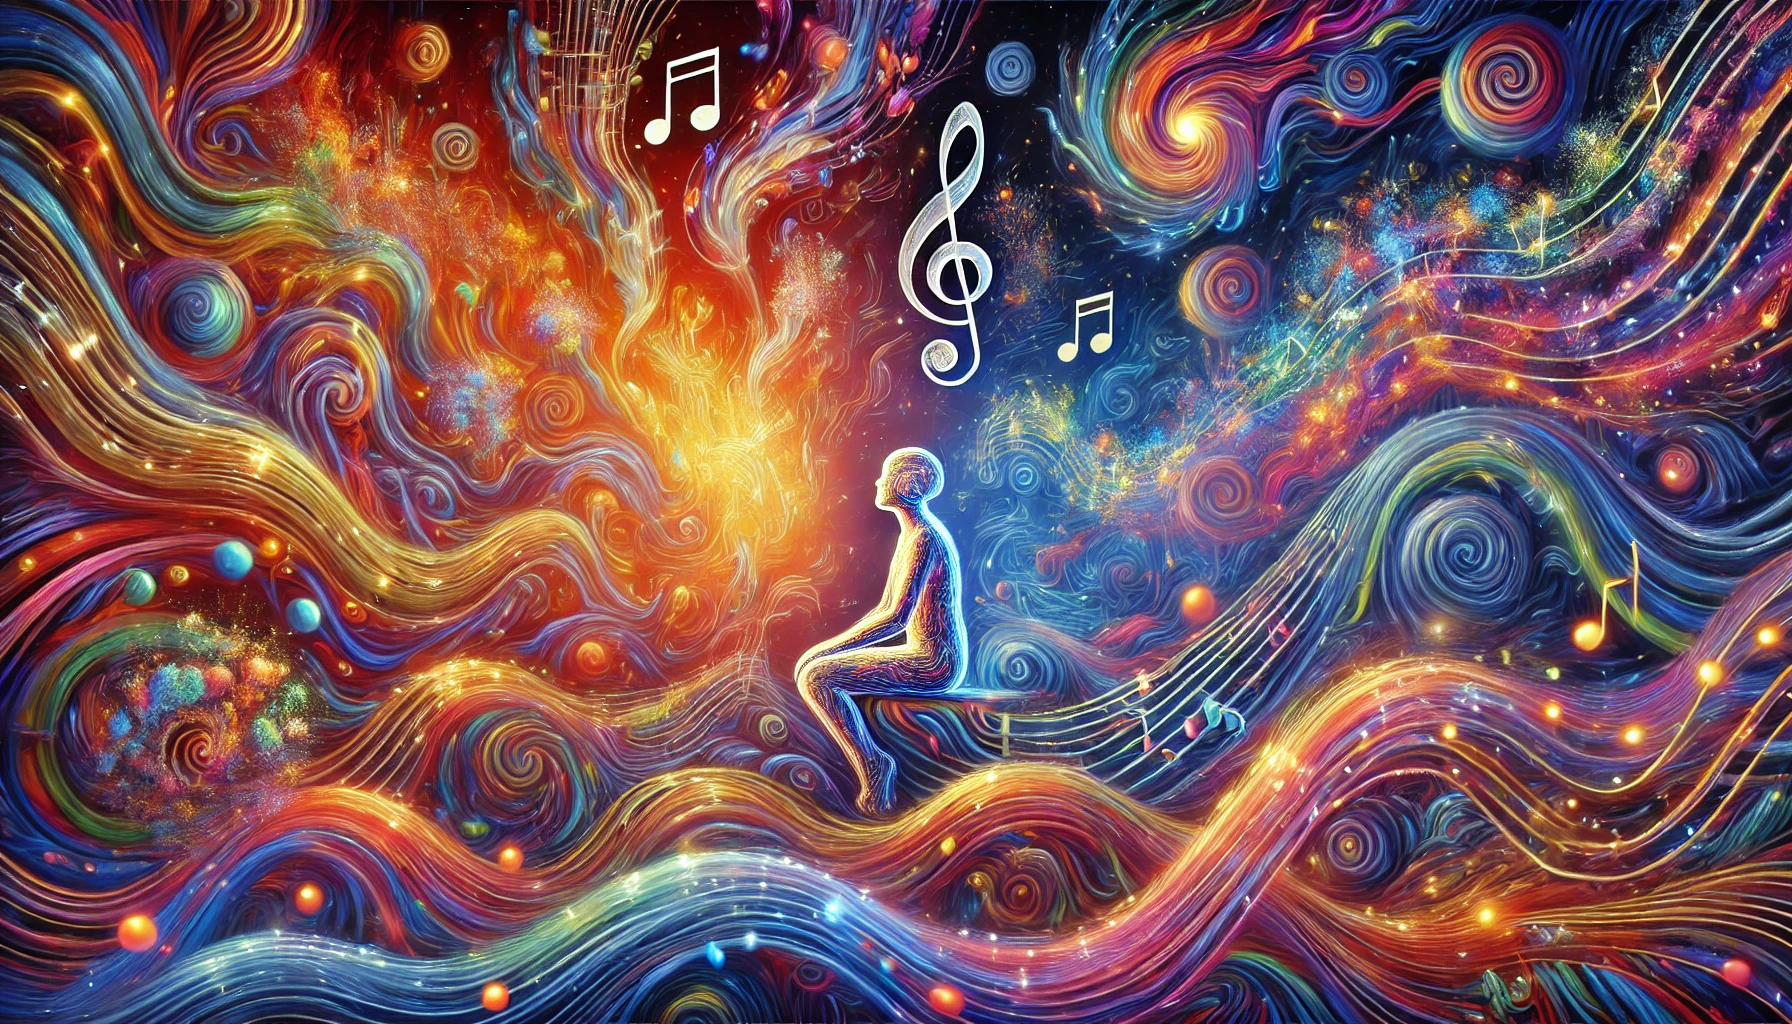
\includegraphics[width=0.8\textwidth]{synaesthesia.png}

    \caption{Synaesthesia - an interplay of senses}
\end{figure}

The study of synaesthetic development reveals crucial insights about how consciousness establishes stable patterns of sensory integration \cite{Barnett2008}. These cross-modal associations typically emerge during critical periods of brain development, when neural plasticity allows for the establishment of novel patterns of sensory integration. The timing and progression of synaesthetic development demonstrates how consciousness relies on specific biological conditions to establish and maintain coherent patterns of cross-modal experience.

The directionality of synaesthetic associations proves particularly revealing about conscious organization \cite{Eagleman2009}. While a grapheme might consistently trigger a specific color experience, the reverse typically does not occur - colors do not automatically evoke specific letters or numbers. This asymmetry suggests that consciousness maintains specific hierarchies in sensory integration, even when establishing novel patterns of cross-modal association. The resulting organizational principles demonstrate how consciousness preserves certain fundamental constraints while enabling novel forms of sensory integration.

Individual differences in synaesthetic experience reveal important principles about conscious variation \cite{Dixon2004}. While some synaesthetes experience vivid, externally projected associations, others describe more subtle, internally experienced connections. These variations in phenomenal quality demonstrate how consciousness can maintain different degrees of perceptual integration while preserving the stability and consistency characteristic of synaesthetic experience.

The relationship between synaesthesia and broader cognitive function reveals sophisticated principles of neural organization \cite{Kadosh2007}. Synaesthetes often demonstrate enhanced memory for information related to their cross-modal associations, suggesting that these additional patterns of sensory integration can support rather than interfere with cognitive processing. This cognitive enhancement demonstrates how novel patterns of conscious organization can provide functional advantages while maintaining coherent processing.

Neural imaging studies of synaesthetes reveal specific patterns of brain activity that correspond to their unique sensory experiences \cite{Nunn2002}. These activation patterns demonstrate how consciousness can establish stable forms of cross-modal integration through specific modifications of neural architecture. The resulting patterns of brain activity reveal how consciousness achieves novel forms of sensory integration through precise alterations in neural organization rather than random cross-activation.

The interaction between synaesthetic experiences and attention reveals sophisticated principles of conscious control \cite{Mattingley2001}. While synaesthetic associations occur automatically, their intensity and salience can be modulated by attentional focus. This relationship demonstrates how consciousness can maintain stable patterns of cross-modal integration while enabling dynamic control over their expression.

The implications of synaesthesia for understanding consciousness extend beyond individual cases to fundamental principles about neural organization \cite{Ramachandran2001}. The ability of consciousness to maintain stable cross-modal associations while preserving normal sensory processing demonstrates remarkable sophistication in managing multiple streams of sensory information. This capacity for parallel processing reveals how consciousness can establish novel patterns of integration while maintaining essential functional organization.

The functional diversity of synaesthetic experience reveals fundamental organizing principles of conscious processing \cite{Grossenbacher2001}. Different forms of synaesthesia utilize distinct patterns of neural connectivity to achieve specific types of cross-modal integration while maintaining broader perceptual coherence. This architectural specialization demonstrates how biological systems can achieve both local specificity and global integration through precise patterns of neural organization \cite{Ward2013}.

Perhaps most significantly, synaesthesia demonstrates how consciousness emerges from specific patterns of neural architecture that enable stable forms of cross-modal integration \cite{Hubbard2005}. Rather than representing mere associations or learned connections, synaesthetic experiences reveal how particular configurations of neural organization can create reliable and consistent forms of conscious experience. This understanding suggests new approaches to studying both normal sensory processing and potential therapeutic applications based on enhancing sensory integration.

In the spirit of expanding on non-standard experiences in the general population, we will now delve deeper into peculiar conditions of the visual field such as visual snow and tetrachromacy.

\section{Visual Snow}

Visual snow offers a unique window into how ECC's framework can explain perceptual phenomena that challenge traditional computational models of consciousness. This condition, characterized by continuous visual static perceived across the entire visual field \cite{Puledda2020}, provides compelling evidence for how consciousness emerges from and remains grounded in underlying patterns of energetic coherence.

The phenomenon demonstrates several key principles of ECC's framework. Unlike typical visual processing, which involves organized patterns of neural activity representing external stimuli, visual snow appears to reveal the background energy dynamics that typically remain below the threshold of conscious awareness. This aligns with evidence suggesting that visual snow may represent a fundamental dysrhythmia in thalamocortical circuits \cite{Lauschke2016}, affecting how the brain maintains coherent visual representations.

Recent clinical investigations have established visual snow as a distinct neurological condition rather than merely a symptom of other disorders \cite{Schankin2014}. The persistence of visual static across different lighting conditions and its independence from external stimuli suggest that it emerges from alterations in how the brain maintains coherent visual states rather than from disruptions in early sensory processing \cite{Bessero2014}.

Through ECC's framework, visual snow can be understood as a modification in how the brain achieves and maintains coherent energy states in visual processing regions. The continuous, grainy quality of the phenomenon reflects underlying patterns of energetic activity that normally remain integrated into seamless visual experience. This interpretation aligns with predictive processing accounts of perception \cite{Clark2013}, suggesting that visual snow represents a disruption in how the brain maintains stable perceptual predictions through coherent energy dynamics.

The relationship between visual snow and other perceptual phenomena becomes particularly clear through ECC's emphasis on energetic coherence. The frequent co-occurrence of persistent after-images and enhanced pattern sensitivity in visual snow patients \cite{Puledda2020} suggests broader alterations in how visual processing regions maintain coherent states. These associated symptoms indicate that visual snow involves fundamental changes in how the brain organizes visual experience through patterns of energetic coherence rather than simple sensory disruption.

This understanding has important implications for both theoretical models of consciousness and clinical approaches to visual snow. Rather than treating the condition as a processing error or pathological activation, ECC suggests it represents an alternative configuration of how consciousness organizes visual experience through energetic coherence. This perspective aligns with embodied approaches to perception \cite{ORegan2001} while providing a specific mechanism - disrupted patterns of energetic coherence - through which altered visual experiences can emerge.

The framework also suggests why visual snow proves resistant to traditional treatments targeting neurotransmitter systems. If the condition represents a fundamental reorganization of how visual regions maintain coherent states, interventions (should they even be required or desired) may need to focus on restoring appropriate patterns of energetic coherence rather than simply modulating neural activity. This understanding could guide the development of new therapeutic approaches based on supporting stable patterns of visual coherence.

Visual snow thus serves as a crucial test case for understanding how consciousness emerges from patterns of energetic coherence in neural systems. The condition demonstrates both the flexibility and constraints of conscious visual processing while suggesting new approaches to investigating and treating disorders of perceptual organization.

\begin{figure}[h]
    \centering
    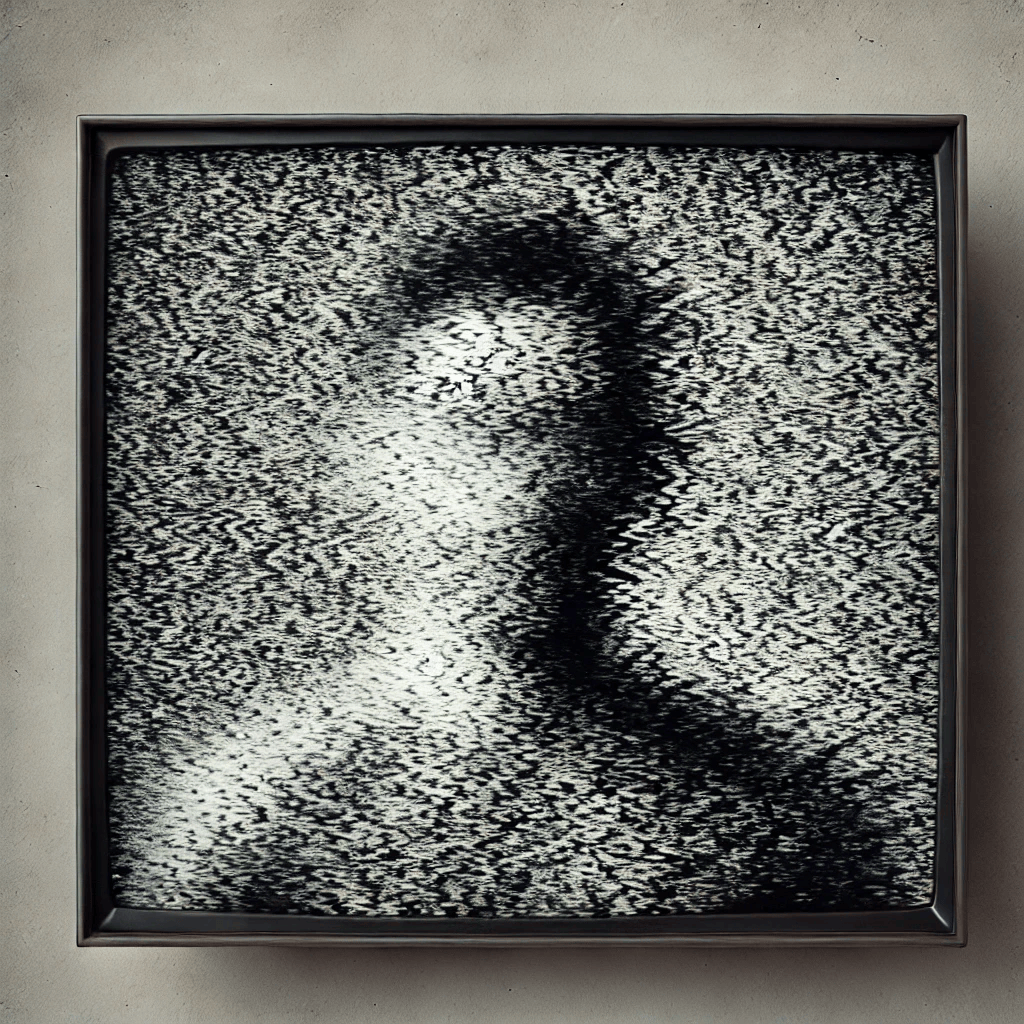
\includegraphics[width=0.8\textwidth]{snow.png}

    \caption{An exaggerated depiction of visual snow.}
\end{figure}

Building on this foundation, we can further explore how visual snow illuminates fundamental principles of perceptual organization through the lens of energetic coherence. Traditional predictive coding accounts \cite{Rao1999, Friston2009} suggest that perception emerges from hierarchical prediction processes, but ECC extends this understanding by grounding these processes in patterns of energetic coherence that maintain stable perceptual states.

The phenomenology of visual snow provides crucial insights into how consciousness maintains coherent perceptual fields. Rather than representing random noise in visual processing, the consistent and organized nature of visual snow - its characteristic density, temporal dynamics, and field-like distribution - suggests disruption in how the brain maintains background patterns of energetic coherence. This aligns with enactive approaches to perception \cite{Varela1991} while providing specific mechanisms through which perceptual experiences emerge from neural dynamics.

Recent theoretical work in sensorimotor contingencies \cite{Seth2014} helps explain why visual snow remains relatively stable across different viewing conditions and contexts. Unlike hallucinations or other visual phenomena that vary with attention or environmental conditions, visual snow maintains consistent characteristics that suggest fundamental alterations in how visual consciousness achieves coherent organization. This stability points to changes in the underlying energetic patterns that support visual experience rather than disruptions in higher-level processing.

The relationship between visual snow and broader theories of consciousness becomes particularly clear when considering how the condition affects perceptual presence - the sense that perceived objects are real and present in the environment \cite{Seth2014}. While visual snow patients maintain normal perception of external objects, the constant presence of visual static reveals how consciousness simultaneously maintains multiple layers of perceptual organization through distinct patterns of energetic coherence.

This multi-level organization of visual consciousness aligns with philosophical accounts of perception that emphasize its active, constitutive nature \cite{Noe2004}. Visual snow demonstrates how consciousness doesn't simply process sensory inputs but actively maintains coherent perceptual states through sophisticated patterns of energetic organization. The condition reveals these organizational processes by making typically implicit aspects of visual processing explicitly present in consciousness.

The theoretical significance of visual snow extends beyond clinical understanding to fundamental questions about the nature of conscious perception. The condition challenges purely representational theories of consciousness \cite{Metzinger2003} by demonstrating how perceptual experience emerges from and remains grounded in patterns of energetic coherence rather than abstract information processing. This suggests new approaches to investigating both normal perception and its alterations in various conditions.

The relationship between visual snow and other perceptual variations provides deeper insight into how consciousness maintains coherent visual states through patterns of energetic organization. Much like color perception demonstrates structured relationships that resist arbitrary reconfiguration \cite{Palmer1999}, visual snow reveals fundamental aspects of how visual consciousness achieves stable organization through coherent energy dynamics.

This perspective aligns with research suggesting that perception emerges from structured relationships within neural systems rather than arbitrary mappings between stimuli and experience \cite{Thompson1995}. Visual snow demonstrates how these relationships can be systematically altered while maintaining basic coherence - the visual static remains organized and stable even as it modifies normal visual experience. This structured modification suggests that consciousness operates through constrained patterns of energetic coherence rather than through unconstrained information processing.

The condition also illuminates debates about the plasticity of perceptual categories \cite{VanBrakel1993}. While visual snow represents a dramatic alteration in visual experience, it maintains consistent characteristics across individuals and contexts, suggesting fundamental constraints on how consciousness can organize visual experience through patterns of energetic coherence. These constraints help explain both the stability of normal perception and the specific ways it can be altered in various conditions.

Understanding visual snow through ECC's framework provides new perspective on classical problems in philosophy of perception, such as the relationship between subjective experience and neural activity \cite{Tye2000}. Rather than requiring a solution to the hard problem of consciousness, ECC suggests that visual snow reveals how conscious experience emerges directly from patterns of energetic coherence in neural systems. This helps explain both the phenomenal character of visual snow and its resistance to reduction to purely computational descriptions.

The implications extend beyond theoretical understanding to practical approaches for investigating and treating perceptual disorders. By recognizing how visual snow emerges from altered patterns of energetic coherence rather than simple processing disruptions, researchers and clinicians might develop more effective interventions focused on restoring appropriate patterns of perceptual organization. This could lead to novel therapeutic approaches that target the underlying organizational principles of visual consciousness rather than just its surface manifestations.

Visual snow thus serves as a crucial case study for understanding how consciousness emerges from and maintains coherent perceptual states through sophisticated patterns of energetic organization. The condition reveals fundamental principles about how consciousness operates while suggesting new directions for both theoretical research and clinical practice. This understanding helps bridge the gap between subjective experience and neural dynamics while providing concrete approaches to investigating and treating disorders of conscious perception.

\section{Color perception}

Color perception, like visual snow, also presents a unique challenge for theories of consciousness, revealing fundamental principles about how neural systems achieve coherent representations of sensory qualities. The apparent universality of certain aspects of color experience, combined with clear evidence of cultural and individual variation \cite{Davidoff2015}, provides crucial insight into how consciousness maintains stable perceptual states while allowing for structured variation.

Recent advances in understanding the biological basis of color perception \cite{ConwayLivingstone2021} demonstrate how specific neural architectures support the emergence of coherent color experiences. Through ECC's framework, these neural mechanisms can be understood not as merely computing color values, but as maintaining specific patterns of energetic coherence that give rise to stable color experiences. This perspective helps bridge the gap between neurobiological mechanisms and phenomenal experience.

The question of color categorization proves particularly revealing about how consciousness organizes perceptual experience. While early theories suggested universal bases for color categories, contemporary research reveals a more complex picture \cite{KayRegier2003}. Cross-cultural studies demonstrate both systematic commonalities and significant variations in how different societies organize color experience \cite{MacLaury1997}. Through ECC's framework, these patterns can be understood as emerging from the interaction between shared biological constraints on energetic coherence and culturally shaped patterns of perceptual organization.

The investigation of color vision in carriers of anomalous trichromacy provides crucial evidence about how conscious color experience emerges from patterns of neural organization \cite{JordanMollon1993}. These studies reveal how variations in photopigment genes can create subtle but significant differences in color discrimination, suggesting that conscious color experience depends on specific patterns of energetic coherence shaped by molecular-level variations in neural architecture.

Traditional color vision theory focused primarily on the three standard cone types, but research has revealed greater complexity in how the visual system achieves coherent color representations. The discovery of individuals with enhanced color discrimination capabilities \cite{Jameson2001} demonstrates how consciousness can maintain more sophisticated patterns of color differentiation when supported by appropriate neural architecture. This aligns with ECC's emphasis on how conscious experiences emerge from specific patterns of energetic coherence rather than abstract computational processes.

Through ECC's framework, color perception can be understood as emerging from structured patterns of energetic coherence that remain stable across individuals while allowing for systematic variation. This helps explain both the commonalities in color experience across cultures and the specific ways that color perception can vary between individuals and populations. The framework suggests that color experience is neither purely subjective nor simply determined by wavelength detection, but emerges from sophisticated patterns of neural organization that support coherent perceptual states.

The relationship between color perception and consciousness thus reveals fundamental principles about how phenomenal experiences emerge from neural dynamics. Rather than requiring a solution to the traditional mind-body problem, ECC suggests that color experiences arise directly from patterns of energetic coherence maintained by specialized neural architectures. This understanding helps explain both the stability and variability of color perception while suggesting new approaches to investigating perceptual consciousness.

Examining how color experience achieves stability while maintaining flexibility provides crucial insight into consciousness itself. Research on color relationalism suggests that perceptual qualities emerge not from simple stimulus-response mappings but from structured relationships within neural systems \cite{ByrneHilbert2017}. Through ECC's framework, these relationships can be understood as patterns of energetic coherence that support stable yet flexible color experiences.

The geometry of color perception proves particularly revealing about how consciousness organizes sensory experiences. Recent mathematical analyses of homogeneous color spaces \cite{Provenzi2020} demonstrate that color experience exhibits intrinsic structural constraints that cannot be reduced to arbitrary mappings. These geometric properties suggest fundamental principles about how consciousness achieves coherent perceptual states through specific patterns of energetic organization. They reveal intrinsic asymmetries and structural relationships that challenge traditional philosophical thought experiments like the inverted spectrum hypothesis \cite{Block1990}. The geometric constraints shown by this line of research suggest that color experiences cannot be arbitrarily inverted or reorganized while maintaining coherent relationships between perceptual qualities and their underlying neural dynamics.

The investigation of color categorization across cultures \cite{Kay2003} mentioned above further illuminates how consciousness achieves stable organization within these geometric constraints. While cultural variations exist in color naming and categorization, these differences operate within structural limitations imposed by the architecture of human color perception. Through ECC's framework, these patterns can be understood as emerging from fundamental constraints on how consciousness can maintain coherent perceptual states.

Research on synaesthetic experiences involving color \cite{HarrisonBaronCohen1997} provides additional insight into how consciousness integrates chromatic information with other perceptual qualities. The systematic nature of color-based synaesthesia suggests that even novel associations between sensory modalities must respect underlying geometric constraints in how consciousness organizes color experience. This structured flexibility demonstrates how consciousness maintains coherent perceptual states while enabling diverse patterns of sensory integration.

The philosophical implications of these findings extend beyond specific questions about color perception to fundamental issues in consciousness studies \cite{Palmer1999}. The existence of geometric constraints on color experience, combined with evidence from tetrachromacy and cross-cultural research, suggests that conscious experiences emerge from structured patterns of energetic coherence that cannot be arbitrarily reorganized. This challenges both radical relativist accounts of perception and simple computational models of consciousness.

Evolutionary considerations highlight how color consciousness emerges from specific neural architectures shaped by biological constraints. The development of trichromatic vision in primates \cite{Neitz2017} demonstrates how consciousness achieves coherent color representation through specialized neural mechanisms that support specific patterns of energetic organization. This evolutionary perspective helps explain both the commonalities in color experience across individuals and the specific ways it can vary between species.

Comparative studies reveal remarkable diversity in how different organisms achieve coherent color representation. Research on avian tetrachromacy \cite{Wilkins2020} demonstrates how neural systems can support forms of color consciousness that transcend human perceptual capabilities. These findings align with ECC's emphasis on how conscious experiences emerge from specific patterns of energetic coherence rather than abstract computational processes.

The investigation of anomalous color vision provides additional insight into how consciousness maintains coherent perceptual states. Studies of individuals with variant photopigment genes \cite{Jordan2010} reveal how subtle alterations in neural architecture can create systematic differences in color experience while maintaining overall perceptual coherence. This demonstrates how consciousness achieves stable color representation through sophisticated patterns of energetic organization that can accommodate significant variation in underlying neural mechanisms.

The relationship between color perception and neural architecture reveals fundamental principles about how consciousness emerges from biological systems. Rather than representing arbitrary mappings between stimuli and sensations, color experience reflects sophisticated patterns of energetic coherence shaped by both evolutionary history and individual development. This understanding helps bridge the gap between subjective experience and neural dynamics while suggesting new approaches to investigating perceptual consciousness.

The dimensionality of color vision takes on particular significance when examined through ECC's framework. Research on the biological basis of color discrimination \cite{Jacobs2018} demonstrates how neural systems achieve coherent representation of multiple color dimensions through specific patterns of energetic organization. This multidimensional organization helps explain both the richness of color experience and the specific constraints on how consciousness can represent chromatic relationships.

The implications of color perception research extend beyond individual variation to fundamental questions about the structure of conscious experience. The study of tetrachromacy, particularly in individuals possessing multiple opsin genes \cite{Jameson2001}, reveals how expanded color perception requires not just additional photoreceptors but appropriate neural architecture to support coherent representation of an enhanced perceptual space. This demonstrates how conscious experiences emerge from specific patterns of energetic coherence that must maintain stability across multiple perceptual dimensions.

Through this lens, color perception emerges not as a simple mapping between wavelengths and sensations, but as a sophisticated achievement of consciousness operating within specific geometric and biological constraints. The stability of color relationships, the possibility of enhanced color vision through tetrachromacy, and the structured nature of cultural variations all point to fundamental principles about how consciousness maintains coherent perceptual states through patterns of energetic organization that respect intrinsic geometric constraints.

This understanding helps resolve longstanding debates about the nature of color experience while suggesting new approaches to investigating consciousness itself. Rather than requiring either pure objectivism about color or complete perceptual relativism, ECC suggests how structured patterns of energetic coherence can give rise to stable yet flexible perceptual experiences that remain grounded in physical reality while allowing for systematic variation between individuals and across cultures.

\section{Music and Auditory Experience}

The relationship between music and consciousness reveals fundamental principles about how neural systems achieve and maintain coherent experiential states across time. Unlike static perceptual experiences, music requires the brain to organize complex temporal patterns while integrating multiple streams of auditory information into unified conscious experiences \cite{Janata2002}. Through ECC's framework, these musical experiences can be understood as emerging from sophisticated patterns of energetic coherence that span multiple temporal and processing scales.

Recent research in music cognition demonstrates how neural systems achieve this temporal integration through dynamic attending processes \cite{Large1999}. Rather than simply processing sequential auditory events, the brain actively maintains coherent states that enable prediction and anticipation of musical patterns. This aligns with ECC's emphasis on how consciousness emerges from organized patterns of energetic coherence rather than mere information processing.

The relationship between music and emotion proves particularly revealing about how consciousness maintains coherent experiential states. Studies of musical emotion demonstrate that affective responses emerge through complex interactions between neural systems \cite{Thompson2010}, suggesting that musical experiences involve patterns of energetic coherence that span both auditory processing and emotional regulation networks. This multi-level integration helps explain music's remarkable capacity to evoke powerful emotional responses while maintaining coherent perceptual organization.

Cross-cultural research in music cognition \cite{Patel2010} reveals both universal patterns and cultural variations in how consciousness organizes musical experience. While certain aspects of musical processing appear to reflect shared biological constraints, the specific ways that different cultures organize musical experience demonstrate how consciousness can achieve coherent states through various patterns of energetic organization. This structured flexibility aligns with ECC's emphasis on how conscious experiences emerge from specific yet variable patterns of neural coherence.

The neural architecture supporting musical experience demonstrates remarkable sophistication in maintaining coherent states across multiple processing streams \cite{Zatorre2007}. Studies of music perception and production reveal how the brain coordinates auditory, motor, and emotional systems through precise temporal relationships. These coordinated patterns of neural activity can be understood through ECC as creating stable yet dynamic fields of conscious experience that enable both perception and performance of music.

Recent theoretical work on embodied music cognition \cite{Krueger2009} suggests that musical experiences emerge from active engagement rather than passive processing. This aligns with ECC's framework by emphasizing how consciousness achieves coherent musical states through dynamic patterns of organization that span perception, action, and emotional response. The resulting integration helps explain both the immediacy of musical experience and its capacity to coordinate complex behavioral responses.

Musical rhythm and entrainment provide particularly clear examples of how consciousness maintains coherent states through time \cite{Clayton2005}. The brain's capacity to synchronize neural activity with musical patterns demonstrates sophisticated mechanisms for achieving temporal coherence across multiple processing scales. These mechanisms support both perception of musical structure and coordination of motor responses, revealing fundamental principles about how consciousness organizes temporal experience through patterns of energetic coherence.

This understanding of music through ECC's framework suggests new approaches to investigating both normal musical experience and its alterations in various neurological conditions \cite{Schaefer2014}. Rather than focusing solely on information processing or pattern recognition, research might productively examine how different aspects of musical experience emerge from specific patterns of energetic coherence in neural systems. This perspective helps bridge the gap between neurobiological mechanisms and phenomenal experience while suggesting new therapeutic applications for music in clinical settings.

Building on these foundational principles, the biological basis of musical experience reveals sophisticated mechanisms for maintaining coherent states across multiple processing domains \cite{Fitch2015}. The capacity to process complex musical structures while coordinating motor responses and emotional engagement demonstrates how consciousness achieves integration through specific patterns of energetic coherence that span various neural systems.

Research on musical expectation and anticipation \cite{Huron2006} illuminates how consciousness maintains coherent states that extend through time. Rather than simply reacting to auditory input, the brain actively generates predictions about musical development, creating stable yet dynamic patterns of energetic coherence that shape both perception and response. These expectancy dynamics help explain music's capacity to create sustained engagement while enabling sophisticated temporal processing.

The conceptual structure of musical experience provides crucial insight into how consciousness organizes complex perceptual states \cite{Zbikowski2002}. Studies of musical cognition reveal how the brain achieves coherent representation of multiple musical dimensions - pitch, rhythm, timbre, harmony - through sophisticated patterns of neural organization. This multi-dimensional integration demonstrates how consciousness maintains stable yet flexible states that support rich musical experiences.

Investigations of everyday musical experience \cite{DeNora2000} reveal how consciousness integrates musical perception with broader aspects of human experience. The capacity of music to shape emotional states, coordinate social behavior, and influence cognitive processing suggests that musical consciousness emerges from patterns of energetic coherence that span multiple domains of experience. This ecological perspective helps explain music's pervasive influence on human behavior and experience.

The neuroscience of musical processing \cite{Peretz2005} demonstrates how different aspects of musical experience emerge from coordinated activity across multiple brain regions. Rather than residing in a single processing stream, musical consciousness involves sophisticated patterns of integration across auditory, motor, emotional, and cognitive systems. Through ECC's framework, these patterns can be understood as creating stable fields of conscious experience that enable complex musical behaviors and responses.

Research on deep listening and altered states in music \cite{Becker2004} reveals how musical experience can fundamentally reshape patterns of conscious organization. The capacity of certain musical practices to induce profound alterations in consciousness suggests that music can directly influence how the brain maintains coherent states. This aligns with ECC's emphasis on how consciousness emerges from specific patterns of energetic organization that can be systematically modified through structured sensory input.

The embodied nature of musical experience \cite{Reybrouck2005} takes on particular significance when examined through ECC's framework. Musical perception involves not just auditory processing but active engagement through motor systems, emotional responses, and cognitive interpretation. This multi-level integration demonstrates how consciousness achieves coherent states through patterns of energetic organization that span the entire brain-body system.

The integration of musical experience with broader cognitive processes illuminates fundamental principles about conscious organization. Studies of auditory-motor interactions in music \cite{Zatorre2007} reveal how consciousness maintains coherent states that span perception and action. This integration demonstrates how musical experience emerges not from passive processing but from active patterns of energetic coherence that coordinate multiple neural systems.

The varieties of musical experience \cite{Bharucha2006} provide crucial insight into how consciousness achieves different forms of coherent organization. From basic rhythm perception to complex harmonic analysis, musical consciousness demonstrates remarkable flexibility in maintaining stable yet sophisticated patterns of energetic coherence. This structured variation helps explain both the universality of certain musical features and the tremendous diversity of musical traditions across cultures.

Through ECC's framework, the temporal dynamics of musical attention \cite{Large1999} take on particular significance. The brain's capacity to track multiple time-varying events while maintaining coherent musical experiences demonstrates sophisticated mechanisms for organizing conscious states across different temporal scales. This temporal integration helps explain how music can create sustained patterns of engagement while supporting complex forms of prediction and anticipation.

The relationship between music and language processing \cite{Patel2010} reveals shared principles about how consciousness organizes temporal patterns. Both domains require the maintenance of coherent states across time, yet music demonstrates distinctive forms of temporal organization that extend beyond linguistic structure. This comparison helps illuminate how consciousness achieves different forms of temporal coherence through specific patterns of neural organization.

Recent work on musical semantics \cite{Reybrouck2005} suggests that meaning in music emerges from structured relationships within conscious experience rather than arbitrary associations. Through ECC's framework, these meaningful relationships can be understood as emerging from specific patterns of energetic coherence that link auditory processing with emotional and cognitive systems. This integrated understanding helps explain both the immediacy and complexity of musical meaning.

The therapeutic applications of music \cite{Schaefer2014} take on new significance when understood through ECC's framework. Music's capacity to influence consciousness through structured patterns of auditory input suggests mechanisms for therapeutic intervention based on restoring or modifying patterns of energetic coherence. This understanding helps explain both the broad efficacy of music therapy and its specific applications in different clinical contexts.

In conclusion, musical experience demonstrates how consciousness achieves coherent organization through sophisticated patterns of energetic integration that span multiple neural systems and temporal scales. This understanding not only illuminates the nature of musical consciousness but suggests fundamental principles about how conscious experience emerges from structured patterns of neural activity. Through careful analysis of musical experience, we gain crucial insight into both the flexibility and constraints of conscious organization in biological systems.

\section{Pain and Arousal}

Pain and arousal represent fundamental shifts in conscious states that illuminate crucial aspects of how consciousness maintains faithful representation through coherent energy dynamics. Recent advances in understanding pain mechanisms \cite{Apkarian2005} demonstrate how neural systems achieve both precise discrimination and motivational salience through specific patterns of energetic organization. These experiences reveal how consciousness maintains coherent states while representing essential information about bodily integrity and environmental demands.

The neural architecture of pain processing reveals sophisticated mechanisms for maintaining coherent conscious states \cite{Tracey2007}. Rather than simply signaling tissue damage, pain involves complex interactions between sensory, emotional, and cognitive systems that create stable yet dynamic patterns of experience. This integration demonstrates how consciousness achieves faithful representation of bodily states through specific patterns of energetic coherence that span multiple processing domains.

Research on the affective dimension of pain \cite{Price2000} illuminates how consciousness maintains coherent states that combine sensory discrimination with emotional significance. Pain experiences emerge from coordinated activity across neural networks that process both the physical properties of noxious stimuli and their emotional implications. This dual processing reflects fundamental principles about how consciousness organizes experiences that demand immediate attention and response.

The relationship between pain and interoception provides crucial insight into how consciousness monitors bodily states \cite{Craig2003}. Pain represents a sophisticated form of conscious awareness that integrates multiple streams of information about physiological condition. Through ECC's framework, these interoceptive experiences can be understood as emerging from specific patterns of energetic coherence that maintain faithful representation of bodily states.

Contemporary understanding of pain mechanisms \cite{Garland2012} suggests that conscious pain experiences emerge from complex interactions between bottom-up sensory processing and top-down modulatory systems. This bidirectional organization demonstrates how consciousness achieves coherent pain states through dynamic patterns of integration that enable both precise discrimination and adaptive regulation.

Arousal systems demonstrate equally sophisticated organization in maintaining conscious states \cite{Pfaff2006}. Through precise regulation of neural activity across multiple systems, the brain achieves different levels of conscious arousal while maintaining coherent organization. This capacity for graded activation demonstrates how consciousness modulates its overall state through specific patterns of energetic coherence.

The cultural dimensions of pain experience \cite{Morris1991} reveal how consciousness integrates biological imperatives with learned interpretations. While pain's basic architecture reflects fundamental biological constraints, its expression and interpretation demonstrate remarkable cultural variation. This structured flexibility aligns with ECC's emphasis on how consciousness achieves coherent states through patterns of organization that combine universal features with learned modifications.

Building on this foundation, research on pain modulation reveals sophisticated mechanisms for maintaining coherent states under varying conditions \cite{Wiech2008}. The brain's capacity to modify pain experience through attentional and emotional processes demonstrates how consciousness achieves flexible regulation while maintaining faithful representation of threatening stimuli. This dynamic control reflects fundamental principles about how consciousness organizes experiences through patterns of energetic coherence.

The relationship between pain and reward systems \cite{Fields2007} illuminates how consciousness maintains coherent states across different motivational domains. Pain processing involves not just aversive signaling but complex interactions with reward circuits that shape behavioral responses. Through ECC's framework, these interactions can be understood as creating stable patterns of energetic coherence that guide adaptive behavior while maintaining accurate representation of bodily states.

Contemporary theories of emotional processing \cite{Barrett2009} suggest that affective experiences, including pain, emerge from fundamental patterns of neural organization rather than simple stimulus-response mappings. Pain experiences demonstrate how consciousness achieves coherent representation through specific patterns of energetic organization that integrate sensory, emotional, and cognitive processing into unified conscious states.

The neuroscience of arousal regulation \cite{Saper2010} reveals how consciousness maintains different levels of activation while preserving coherent organization. Sleep-wake transitions and varying states of alertness demonstrate how consciousness modulates its overall energetic state through sophisticated patterns of neural coordination. This capacity for regulated state transitions proves essential for maintaining adaptive conscious processing across different behavioral contexts.

Research on the relationship between pain and consciousness \cite{Damasio2013} demonstrates how conscious experiences emerge from patterns of neural activity that represent both current bodily states and their implications for future action. Pain's dual nature as both sensation and motivation reflects fundamental principles about how consciousness organizes experiences that require immediate awareness and response.

The evolutionary significance of pain and arousal systems \cite{Melzack1965} helps explain their fundamental role in conscious organization. These systems reflect ancient mechanisms for maintaining coherent representation of threats and opportunities while enabling appropriate behavioral responses. Through ECC's framework, these evolutionary constraints can be understood as shaping how consciousness achieves coherent states through specific patterns of energetic organization.

The relationship between arousal and cognitive performance, first formalized in the Yerkes-Dodson law \cite{Yerkes1908}, reveals fundamental principles about how consciousness maintains optimal states through specific patterns of energetic coherence. Different cognitive tasks require different levels of arousal for optimal performance, demonstrating how consciousness achieves effective organization through precise regulation of its energetic states.

Research on pain chronification \cite{Tracey2007} illuminates how persistent pain can fundamentally reshape patterns of conscious organization. Unlike acute pain, which maintains adaptive warning functions, chronic pain involves maladaptive changes in how consciousness maintains coherent states across time. This distinction helps explain both the biological utility of normal pain and the devastating impact of its pathological forms.

The integration of pain with broader emotional states \cite{Price2000} demonstrates how consciousness achieves coherent organization across multiple processing domains. Pain experiences involve not just sensory discrimination but complex emotional responses that shape both immediate experience and future behavior. Through ECC's framework, these emotional aspects can be understood as emerging from specific patterns of energetic coherence that span multiple neural systems.

Studies of pain modulation through cognitive processes \cite{Wiech2008} reveal sophisticated mechanisms for maintaining coherent states while enabling adaptive regulation. The brain's capacity to modify pain experience through attention, expectation, and emotional context demonstrates how consciousness achieves flexible control while maintaining faithful representation of bodily states. This regulated flexibility proves essential for adaptive functioning in complex environments.

Recent work on the relationship between arousal and attention \cite{Pfaff2006} suggests that consciousness maintains coherent states through careful coordination of multiple regulatory systems. Rather than representing simple activation, arousal involves sophisticated patterns of neural organization that enable both focused attention and broader awareness. This multi-level regulation demonstrates how consciousness achieves effective states through specific patterns of energetic coherence.

From a more speculative perspective (re ECC), pain can be conceptualized as a local disruption in the brain’s multi-scale energy flow, specifically one that propagates a strong dissonant signal through neuronal and astrocytic networks. In ECC’s view, normal conscious processing requires coherent alignment of electromagnetic, chemical, and potentially mechanical parameters across cortical and subcortical regions. Painful stimuli produce an intense concentration of chemical and electrical activity at localized sites (for instance, where nociceptive signals enter the dorsal horn of the spinal cord or ascend to higher brain centers), setting off a cascade of heightened, energetically demanding responses that temporarily destabilize or "pull" the surrounding substrate into an atypical high-energy configuration. This localized disturbance forces the rest of the network to compensate, manifesting as the subjective experience of pain. In other words, pain arises when a mismatch or overload in local energetic fields reverberates through the larger network, producing an emergent feeling of distress.

Arousal, by contrast, may be understood as a generalized, system-wide shift in the baseline of energetic coherence, one that increases the capacity of different brain regions to synchronize quickly and robustly under demands. Whereas pain reflects a potent, localized breach in energetic harmony, a heightened state of arousal aligns the stress-energy dynamics across broader swaths of the brain, effectively priming neural circuits for rapid modulation and integration. From an ECC standpoint, arousal involves elevating the background energy influx, possibly via neuromodulators like norepinephrine or acetylcholine, such that local disruptions and signals can swiftly become integrated into the global energetic field. This heightened readiness ensures that salient stimuli are assimilated almost immediately, leading to rapid conscious access and adaptive response. Thus, while pain represents a localized spike in incoherence radiating outward, arousal reflects an overall amplification of the system’s coherent energetic background, making the network more sensitive and responsive to incoming perturbations.

These insights about pain and arousal extend beyond clinical understanding to fundamental questions about conscious organization. Rather than representing simple warning signals or activation states, pain and arousal demonstrate how consciousness maintains coherent representation of essential biological information through sophisticated patterns of energetic organization. This understanding helps explain both the immediate character of these experiences and their broader influence on conscious states.

Through this analysis, pain and arousal emerge as fundamental aspects of how consciousness maintains effective organization through specific patterns of energetic coherence. These systems demonstrate both the sophistication of conscious regulation and its essential role in maintaining adaptive behavior through faithful representation of bodily states and environmental demands.

% TODO: does a section on Attention make sense here?
% What about pleasure, value & reward?

\section{Emotions and Affective States}

Research in affective neuroscience reveals how emotions emerge from sophisticated patterns of neural organization that integrate multiple processing streams into coherent conscious states \cite{Panksepp1998}. Rather than representing simple responses to stimuli, emotions demonstrate how consciousness achieves complex integration through specific patterns of energetic coherence that span cognitive, physiological, and behavioral systems.

Contemporary theories of emotion \cite{Barrett2017} suggest that affective experiences emerge from fundamental patterns of neural organization rather than discrete, universal categories. Through ECC's framework, emotions can be understood as coherent states that integrate interoceptive information, conceptual knowledge, and situational context into unified conscious experiences. This construction reflects sophisticated principles about how consciousness maintains adaptive organization through specific patterns of energetic coherence.

Cross-cultural research on emotion \cite{Lutz1988} demonstrates both universality and variation in how consciousness organizes affective experience. While certain aspects of emotional processing appear to reflect shared biological constraints, the specific ways that different cultures conceptualize and express emotions reveal how consciousness achieves coherent states through various patterns of energetic organization. This structured flexibility helps explain both the biological foundations of emotion and its cultural elaboration.

The social functions of emotion \cite{Keltner2001} illuminate how affective states coordinate behavior across individuals while maintaining coherent individual experience. Emotions serve not just as internal states but as sophisticated mechanisms for social communication and coordination. Through ECC's framework, these social aspects can be understood as emerging from patterns of energetic coherence that enable both individual experience and interpersonal synchronization.

Recent work on the relationship between emotion and bodily states \cite{Damasio2018} reveals how consciousness maintains faithful representation of organismic conditions through specific patterns of affective organization. Rather than representing purely mental states, emotions emerge from integrated patterns of neural activity that track essential information about bodily conditions and environmental relationships.

The development of emotional regulation capabilities \cite{Siegel2012} demonstrates how consciousness achieves increasingly sophisticated patterns of affective organization through maturation and experience. This developmental trajectory reflects fundamental principles about how consciousness establishes and maintains coherent emotional states through specific patterns of energetic organization that become more refined over time.

Research on the neural architecture of emotion \cite{Davidson2012} reveals how different aspects of affective experience emerge from coordinated activity across multiple brain systems. Rather than residing in dedicated emotional centers, affective states arise from sophisticated patterns of integration that span cognitive, visceral, and motor systems. This distributed organization demonstrates how consciousness achieves coherent emotional states through specific patterns of energetic coherence that coordinate multiple processing streams.

The relationship between emotion and consciousness reveals fundamental principles about how neural systems achieve coherent experiential states. Recent research on emotional granularity \cite{Barrett2017} demonstrates how consciousness can maintain increasingly refined patterns of affective discrimination through specific forms of energetic organization. This capacity for nuanced emotional experience reflects sophisticated mechanisms for maintaining distinct yet related affective states.

Studies of emotional embodiment \cite{Fuchs2019} illuminate how affective states emerge from integrated patterns of neural activity that span brain, body, and environment. Rather than representing purely mental phenomena, emotions demonstrate how consciousness achieves coherent states through patterns of energetic organization that maintain faithful representation of organismic conditions while enabling adaptive responses to environmental demands.

The investigation of emotional development through socialization \cite{Thompson2007} reveals how consciousness establishes increasingly sophisticated patterns of affective organization through experience. This developmental trajectory demonstrates how emotional coherence emerges from specific patterns of neural organization that become more refined through social interaction and cultural learning.

Recent advances in understanding the neuroscience of emotion \cite{Fox2019} suggest that affective states emerge from coordinated activity across multiple neural systems rather than from activity in isolated emotional centers. This distributed processing reveals how consciousness achieves coherent emotional states through patterns of energetic organization that integrate multiple processing streams while maintaining stable experiential qualities.

Work on the cultural construction of emotion \cite{Lutz1988} demonstrates how consciousness achieves coherent affective states through patterns of organization that combine universal biological constraints with learned cultural frameworks. This structured flexibility helps explain both the commonalities in emotional experience across cultures and the specific ways that different societies organize and interpret affective states.

The evolutionary foundations of emotion \cite{Panksepp1998} illuminate how affective states reflect fundamental mechanisms for maintaining adaptive conscious organization. Through specific patterns of energetic coherence, emotions enable rapid yet sophisticated responses to environmental challenges while maintaining coherent representation of organismic needs and social relationships.

The relationship between emotion and social cognition \cite{Scherer2014} reveals how affective states coordinate interpersonal behavior while maintaining individual coherence. Through sophisticated patterns of neural organization, emotions enable both personal experience and social communication, demonstrating how consciousness achieves states that serve both individual and collective functions.

Building on these foundations, research on emotional authenticity and regulation \cite{Ekman2003} reveals how consciousness maintains coherent affective states while enabling sophisticated control. Unlike simple suppression or amplification, emotional regulation involves complex patterns of energetic organization that allow for flexible modulation while preserving essential affective information.

Historical perspectives on emotion \cite{Reddy2001} demonstrate how consciousness achieves coherent affective states through patterns of organization that evolve across both individual development and cultural history. This temporal dimension reveals how emotional coherence emerges from dynamic patterns of neural organization that remain stable enough to support reliable experience while allowing for cultural and historical variation.

Anthropological studies of emotion \cite{Rosaldo1980} illuminate how different societies achieve coherent affective organization through distinct cultural frameworks. While emotions reflect shared biological foundations, their specific manifestations demonstrate how consciousness can maintain coherent states through various patterns of energetic organization shaped by cultural learning and social practice.

The social construction of emotional meaning \cite{White1994} reveals how affective states acquire significance through patterns of organization that integrate personal experience with cultural interpretation. Through ECC's framework, these meaningful relationships can be understood as emerging from specific patterns of energetic coherence that link individual experience with collective understanding.

Contemporary theoretical syntheses \cite{Wentworth1992} suggest that emotions emerge from sophisticated interactions between biological systems, personal history, and social context. Rather than representing either pure biology or pure construction, emotions demonstrate how consciousness achieves coherent states through patterns of organization that integrate multiple levels of influence.

The relationship between emotion and moral experience \cite{LeDoux2015} illuminates how affective states shape fundamental aspects of human consciousness. Through specific patterns of energetic coherence, emotions inform moral judgment and behavior while maintaining stable relationships between personal experience and social values. This integration demonstrates how consciousness achieves states that guide both individual conduct and collective coordination.

Through this analysis, emotions emerge as sophisticated achievements of conscious organization that maintain coherent states while enabling complex adaptation to physical and social demands. Rather than representing simple responses or pure constructions, emotions demonstrate how consciousness achieves effective organization through specific patterns of energetic coherence that integrate multiple processing streams while maintaining faithful representation of essential biological and social information.

\section{Language and Communication}

Language represents a sophisticated mechanism for coordinating conscious states across individuals through structured patterns of energetic coherence. Recent theoretical work \cite{Feldman2008} suggests that language functions not merely as abstract symbol manipulation but as a physical system for inducing corresponding patterns of neural organization across brains. Through ECC's framework, linguistic communication can be understood as a constrained form of "telepathy" that enables precise sharing of mental states while respecting physical limitations on information transfer.

Research on the embodied foundations of language \cite{Barsalou2008} reveals how linguistic meaning emerges from patterns of neural activity grounded in sensorimotor experience. Rather than representing arbitrary symbols, words and grammatical patterns reflect organized configurations of conscious experience that enable reliable communication between individuals. This grounding helps explain both language's remarkable effectiveness and its inherent constraints.

Studies on the evolution of language \cite{Deacon1997} demonstrate how communicative systems emerge from the interaction between biological constraints and cultural development. While certain aspects of language organization reflect shared neural architecture, the tremendous diversity of human languages reveals how consciousness can achieve coherent communicative states through various patterns of energetic organization.

The relationship between gesture and language \cite{GoldinMeadow2003} illuminates how linguistic communication extends beyond vocal-auditory channels to include sophisticated patterns of bodily coordination. This multimodal nature of language demonstrates how consciousness achieves coherent states through integrated patterns of energetic organization that span multiple sensory and motor systems.

Contemporary approaches to linguistic anthropology \cite{Duranti2009} reveal how language systems emerge from complex interactions between biological capacities and cultural practice. While universal features of language reflect shared neural constraints, the specific ways different societies organize linguistic communication demonstrate how consciousness achieves coherent states through culturally shaped patterns of energetic organization.

Research on the neural architecture of language \cite{Pulvermuller2002} suggests that linguistic processing emerges from coordinated activity across distributed brain networks rather than from isolated language centers. This distributed organization reveals how consciousness maintains coherent linguistic states through patterns of energetic coherence that integrate multiple processing streams.

The investigation of language acquisition \cite{Tomasello2008} demonstrates how consciousness develops increasingly sophisticated patterns of linguistic organization through experience. This developmental trajectory reveals fundamental principles about how consciousness establishes and maintains coherent communicative states through specific patterns of energetic organization that become more refined over time.

\begin{figure}[h]
    \centering
    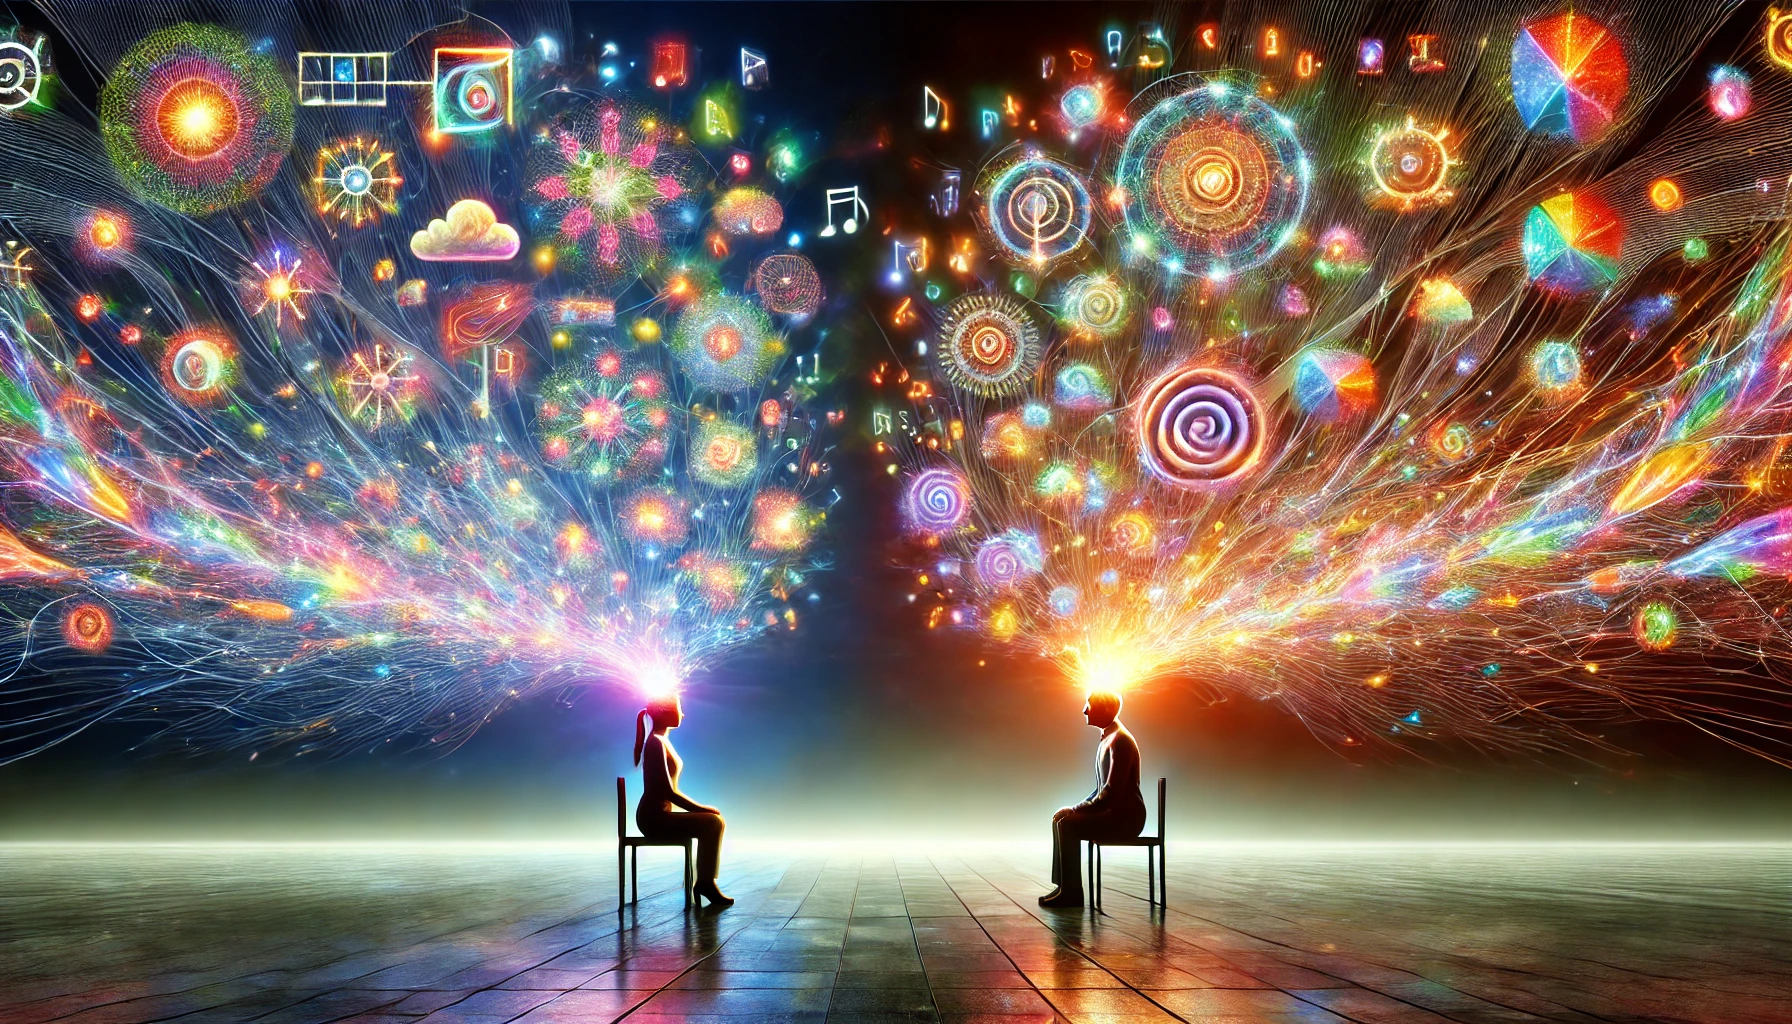
\includegraphics[width=0.8\textwidth]{language.png}

    \caption{Language as a form of telepathy}
\end{figure}

Research on conversational dynamics \cite{Enfield2017} reveals how consciousness achieves coherent states that enable real-time coordination between individuals. The sophisticated timing and turn-taking patterns in conversation demonstrate how consciousness maintains stable yet flexible patterns of organization that support fluid interpersonal communication while respecting physical constraints on information exchange.

The study of conceptual integration in language \cite{Fauconnier2002} illuminates how consciousness combines multiple domains of experience into unified linguistic expressions. This capacity for creative blending reveals how language enables sophisticated forms of conscious organization through specific patterns of energetic coherence that support both stability and innovation in communication.

Work on the origins of human communication \cite{Tomasello2008} suggests that language emerged from more basic forms of social coordination through increasingly sophisticated patterns of neural organization. This evolutionary perspective helps explain both the universal features of language and its unique capacity to support complex forms of conscious coordination between individuals.

Investigations of linguistic anthropology \cite{Silverstein1976} demonstrate how different societies achieve coherent communicative organization through distinct cultural frameworks. While language reflects shared biological foundations, its specific manifestations show how consciousness can maintain coherent states through various patterns of energetic organization shaped by cultural learning and social practice.

Recent theoretical syntheses \cite{Christiansen2016} suggest that language emerges from complex interactions between biological constraints, cognitive development, and cultural evolution. Rather than representing either pure biology or pure construction, language demonstrates how consciousness achieves coherent states through patterns of organization that integrate multiple levels of influence.

Research on brain-to-brain interfaces and linguistic communication \cite{Dingemanse2017} reveals how language enables precise coordination of conscious states across individuals while maintaining physical constraints on information transfer. This perspective helps explain both the remarkable effectiveness of linguistic communication and its inherent limitations.

The relationship between language and thought \cite{Whorf1956} gains new significance when examined through ECC's framework. Rather than simply reflecting or determining thought, language demonstrates how consciousness achieves coherent states through patterns of organization that enable both individual cognition and interpersonal communication.

The embodied nature of linguistic meaning \cite{Lakoff1999} takes on particular significance when examined through ECC's framework. Language works not through abstract symbol manipulation but through patterns of neural organization grounded in physical experience. This embodied foundation helps explain both the stability of linguistic meaning across individuals and the specific ways it can vary between cultures and contexts.

Research on gesture and thought \cite{McNeill2005} demonstrates how linguistic consciousness integrates multiple modalities into coherent communicative states. Rather than being mere supplements to speech, gestures reveal how consciousness achieves coherent expression through patterns of energetic organization that span both vocal and manual channels. This multimodal integration suggests fundamental principles about how consciousness maintains coherent states across different expressive systems.

Studies of language evolution \cite{Hauser2002} reveal how communicative systems emerge from specific patterns of neural organization that enable both individual thought and social coordination. This dual function helps explain why language exhibits both universal features reflecting shared biological constraints and tremendous variation reflecting cultural diversification.

The cultural scaffolding of linguistic consciousness \cite{Vygotsky2012} illuminates how communicative competence develops through structured social interaction. Language acquisition involves not just learning words and rules but developing sophisticated patterns of energetic coherence that enable participation in culturally specific forms of conscious coordination.

The role of language in distributing agency and coordinating social action \cite{Arbib2012} reveals how linguistic communication enables complex forms of collective organization. Through specific patterns of energetic coherence, language supports both individual consciousness and sophisticated forms of group coordination. This capacity for multi-level organization demonstrates how consciousness achieves states that serve both personal and collective functions.

Through this analysis, language emerges as a remarkable system for coordinating conscious states across individuals through specific patterns of energetic organization. Rather than representing arbitrary symbols or pure social construction, language demonstrates how consciousness achieves effective communication through sophisticated patterns of neural coherence that respect both biological constraints and cultural innovation. This understanding helps explain both language's universal features and its remarkable capacity for cultural elaboration.

The investigation of these linguistic principles suggests fundamental insights about consciousness itself - particularly how it maintains coherent states that enable both individual thought and social coordination through physically constrained patterns of energetic organization. This bridge between individual and collective consciousness through language represents one of the most sophisticated achievements of human neural organization.

\section{Math, Logic and Rationality}

Mathematical and logical thinking (i.e., symbolic reasoning) represent sophisticated achievements of conscious organization that require maintaining coherent states detached from immediate sensory experience. Recent work \cite{Lakoff2000} suggests that even abstract mathematical concepts emerge from embodied patterns of neural organization rather than purely symbolic manipulation. Through ECC's framework, mathematical cognition can be understood as requiring specific patterns of energetic coherence that support abstract relationships while remaining grounded in physical neural dynamics.

Research on the cognitive foundations of mathematics \cite{Dehaene2011b} reveals how numerical understanding emerges from basic patterns of neural organization that support quantity discrimination and spatial relationships. Rather than representing purely abstract symbols, mathematical concepts reflect sophisticated organizations of conscious experience that enable precise manipulation of quantitative relationships. This grounding helps explain both mathematics' power and its cognitive demands.

The anthropological study of mathematical practices \cite{Ascher1991} demonstrates how different cultures achieve coherent mathematical understanding through various patterns of organization. While certain aspects of mathematical thinking appear to reflect shared cognitive capacities, the specific ways that different societies develop mathematical concepts reveal how consciousness can achieve abstract coherence through culturally shaped patterns of energetic organization.

Work on the embodied basis of mathematical reasoning \cite{Lakoff2000} illuminates how abstract mathematical concepts emerge from patterns of neural activity grounded in sensorimotor experience. This perspective suggests that even highly abstract mathematics requires maintaining specific patterns of energetic coherence that remain connected to more basic forms of perceptual and motor organization.

The psychology of mathematical invention \cite{Hadamard1945} reveals how consciousness achieves novel mathematical insights through specific patterns of organization that enable creative recombination of existing concepts. This capacity for mathematical creativity demonstrates how consciousness can maintain coherent states that support both stability and innovation in abstract thinking.

Studies of mathematical cognition \cite{Devlin2000} suggest that mathematical ability emerges from coordinated activity across multiple neural systems rather than from an isolated "math module." This distributed organization reveals how consciousness achieves coherent mathematical states through patterns of energetic organization that integrate multiple processing streams while maintaining stable abstract relationships.

The relationship between mathematics and natural language \cite{MacLane1986} takes on new significance when examined through ECC's framework. Rather than representing a purely formal system, mathematics demonstrates how consciousness achieves coherent states through patterns of organization that enable both precise symbolic manipulation and communication of abstract concepts.

The development of mathematical intuition \cite{Penrose1994} reveals how consciousness achieves increasingly sophisticated patterns of abstract organization through experience. Rather than operating through purely formal rules, mathematical understanding emerges from specific patterns of energetic coherence that enable direct grasp of abstract relationships. This intuitive dimension demonstrates how consciousness maintains stable abstract states beyond simple symbol manipulation.

Research on mathematical discovery processes \cite{Lakatos1976} illuminates how new mathematical insights emerge through patterns of organization that combine logical rigor with creative exploration. The dynamic between proof and refutation demonstrates how consciousness achieves coherent mathematical states through patterns of energetic organization that enable both stability and innovation in abstract thinking.

Studies of mathematical enculturation \cite{Lloyd1990} reveal how different societies develop coherent systems of mathematical understanding through cultural practices. While mathematical truth may be universal, the specific ways that different cultures organize mathematical knowledge demonstrate how consciousness achieves abstract coherence through culturally shaped patterns of energetic organization.

Work on personal knowledge in mathematics \cite{Polanyi1958} suggests that mathematical understanding involves tacit dimensions that cannot be reduced to formal rules. This implicit aspect of mathematical knowledge reveals how consciousness maintains coherent abstract states through patterns of organization that extend beyond explicit symbolic representation.

The embodied mind perspective \cite{Varela1991} illuminates how mathematical cognition emerges from patterns of neural organization grounded in physical experience. Rather than representing purely abstract manipulation, mathematical thinking demonstrates how consciousness achieves coherent states through patterns of energetic organization that remain connected to embodied understanding.

Investigation of mathematical practices \cite{Rotman1993} reveals how consciousness maintains abstract coherence while enabling precise manipulation of mathematical relationships. The interplay between intuition and formalism demonstrates how consciousness achieves states that support both creative insight and rigorous proof through specific patterns of energetic organization.

Contemporary research on mathematical cognition \cite{DAmbrosio1985} suggests that mathematical ability emerges from coordinated activity across multiple neural systems. This distributed organization reveals how consciousness maintains coherent mathematical states through patterns of energetic coherence that integrate multiple processing streams.

Scientific understanding of rationality \cite{Gigerenzer2008} suggests that logical thinking emerges not from purely abstract rule-following but from sophisticated patterns of neural organization that enable reliable inference while respecting cognitive constraints. Through ECC's framework, rational thought can be understood as requiring specific patterns of energetic coherence that support abstract reasoning while remaining grounded in biological limitations.

The cultural transmission of mathematical knowledge \cite{Sperber1996} illuminates how abstract thinking develops through structured social interaction. Mathematical learning involves not just mastering formal systems but developing sophisticated patterns of energetic coherence that enable participation in culturally specific forms of abstract reasoning. This perspective helps explain both the universality of basic mathematical concepts and their diverse cultural elaborations.

Research on mathematical intuition \cite{Barrow1992} reveals how consciousness achieves direct grasp of abstract relationships through specific patterns of neural organization. Rather than operating solely through step-by-step deduction, mathematical understanding demonstrates how consciousness maintains coherent states that enable immediate recognition of mathematical truth while supporting rigorous verification.

The investigation of mathematical creativity \cite{Hadamard1945} demonstrates how consciousness generates novel insights through patterns of organization that enable flexible recombination of existing concepts. This creative dimension reveals how consciousness achieves states that support both stability and innovation in abstract thinking through specific patterns of energetic coherence.

Studies of mathematical development \cite{Piaget1952} show how abstract thinking emerges from more basic forms of cognitive organization. This developmental trajectory demonstrates how consciousness establishes increasingly sophisticated patterns of coherence that enable manipulation of abstract relationships while maintaining connection to embodied understanding.

From an ECC standpoint, logic and mathematical reasoning represent cognitively demanding processes precisely because they require the brain to maintain coherence in a domain that is largely "ungrounded" from typical energetic flows. In most conscious activities—such as perceiving the environment, processing emotions, or initiating motor responses—the underlying energetic patterns (electromagnetic fields, chemical gradients, and mechanical forces) correspond more or less directly to concrete features of the world. Logic and mathematics, however, compel the system to detach from these usual grounding points and instead uphold a set of abstract symbolic relationships, which the brain enacts by creating and sustaining new, internally consistent energetic configurations that do not map straightforwardly onto real-world inputs.

This detachment demands significant attentional resources and increased metabolic investment, as multiple brain networks must remain highly synchronized to support the manipulation of placeholders, free variables \footnote{In ECC, free variables are mental representations that can be manipulated independently of immediate physical grounding, enabling abstract thought while requiring active maintenance.}, or purely formal structures rather than intrinsic sensorimotor loops. This partly explains why symbolic reasoning is so effortful and resists parallelization (see \cite{Dehaene2011, kahneman2011thinking}); at least until a learned symbolic procedure can become more automatic.

In line with ECC, learning and engaging in mathematics or logic can be interpreted as a deliberate reorganization of energetic coherence at multiple hierarchical levels: the local fields in relevant cortical areas (prefrontal, parietal, and temporal regions), the global integrative dynamics that unify them, and possibly even transcriptomic or glial mechanisms that underlie adaptive neural plasticity. Early in the process of acquiring a new logical or mathematical skill, the mismatch between abstract reasoning and everyday bodily or perceptual coherence can be substantial, causing fatigue or frustration. Over time, with practice and repetition, certain neural patterns become more stable, reducing the energetic load required to manipulate purely formal concepts. Even so, these abstract tasks remain comparatively resource-intensive relative to more perceptually grounded actions, since sustaining abstract variables requires continuously preventing them from slipping back into more familiar, energetically efficient thought patterns.

Through this analysis, mathematical and logical thinking emerge as sophisticated achievements of conscious organization that require maintaining coherent states detached from immediate experience. Rather than representing purely formal manipulation, mathematical cognition demonstrates how consciousness achieves effective abstract thinking through specific patterns of neural coherence that respect both logical necessity and biological constraints. This understanding helps explain both mathematics' remarkable power and its significant cognitive demands.

The relationship between mathematical thinking and consciousness thus reveals fundamental principles about how neural systems achieve and maintain coherent states that support abstract reasoning while remaining grounded in physical reality. This balance between abstraction and embodiment represents one of the most sophisticated achievements of human conscious organization.

\section{Developmental Psychology and Neuroscience}

Through the lens of ECC, developmental psychology and neuroscience reveal fundamental principles about how conscious processing emerges through increasingly sophisticated patterns of energetic coherence. Recent theoretical work \cite{Bjorklund2014} suggests that cognitive development reflects not just maturation or learning but the progressive refinement of how neural systems maintain coherent conscious states. This developmental trajectory demonstrates how consciousness emerges through specific patterns of organization that become increasingly sophisticated over time.

Research on early brain development \cite{DehaeneLambertz2015} illuminates how neural systems establish basic patterns of coherent organization that support conscious processing. Rather than representing simple maturation, early development involves the careful coordination of multiple processes that create the conditions necessary for conscious experience. This foundation helps explain both the universal features of early development and its sensitivity to environmental input.

Studies of developmental psychopathology \cite{Cicchetti2016} demonstrate how disruptions to normal developmental processes can alter how consciousness achieves and maintains coherent states. These variations in developmental trajectories reveal how conscious organization depends on specific patterns of neural coherence that can be affected by both genetic and environmental factors.

The investigation of self-development \cite{Damasio2010} reveals how consciousness establishes increasingly sophisticated patterns of self-organization through experience. Rather than representing a simple accumulation of knowledge, the development of self-awareness demonstrates how consciousness achieves coherent states that integrate multiple aspects of experience into unified self-representation.

Work on neural plasticity and development \cite{Nelson2021} suggests that conscious capabilities emerge through specific patterns of neural organization that remain flexible throughout development. This plasticity reveals how consciousness maintains stable patterns of organization while enabling adaptation to environmental demands and learning opportunities.

Contemporary approaches to cognitive development \cite{Carey2009} demonstrate how children achieve increasingly sophisticated forms of conscious organization through structured interaction with their environment. This developmental progression reveals how consciousness establishes coherent states through patterns of energetic organization that become more refined through experience.

The relationship between brain development and consciousness \cite{Johnson2011} takes on new significance when examined through ECC's framework. Rather than simply supporting conscious processing, neural development creates the specific patterns of energetic coherence necessary for conscious experience.

Research on neural Darwinism \cite{Edelman1987} reveals how conscious capabilities emerge through selective stabilization of specific patterns of neural organization. This selective process demonstrates how consciousness achieves coherent states through patterns of energetic organization that prove adaptive for the developing organism while remaining flexible enough to incorporate new experiences.

Studies of probabilistic epigenesis \cite{Gottlieb2007} illuminate how conscious development emerges from complex interactions between genetic, neural, and environmental factors. Rather than following a predetermined program, conscious development demonstrates how coherent states emerge through bidirectional influences across multiple levels of organization.

The exploration of developmental motivation \cite{Kagan2013} reveals how consciousness maintains coherent states that guide behavior while enabling learning and adaptation. This motivational framework demonstrates how consciousness achieves states that support both stability and exploration through specific patterns of energetic organization.

Work on self and motivational systems \cite{Lichtenberg2016} suggests that conscious development involves the progressive refinement of how neural systems maintain coherent states that support both individual identity and social engagement. This dual development reveals how consciousness achieves increasingly sophisticated patterns of organization that serve both personal and interpersonal functions.

Research on the birth of mind \cite{Marcus2004} demonstrates how genetic factors shape the basic patterns of neural organization that support conscious processing. This biological foundation helps explain both the universal features of conscious development and the specific ways it can vary between individuals.

Contemporary approaches to psychoanalytic development \cite{Stern2000} reveal how consciousness establishes increasingly sophisticated patterns of emotional and interpersonal organization through early experience. This emotional development demonstrates how consciousness achieves coherent states that integrate affect, cognition, and social understanding.

Dynamic systems approaches \cite{Thelen1996} illuminate how conscious capabilities emerge from the coordinated activity of multiple developing systems. Rather than following a linear trajectory, conscious development demonstrates how coherent states emerge through complex interactions across multiple scales of organization.

The investigation of infant intersubjectivity \cite{Trevarthen2011} reveals how consciousness achieves coherent states that enable social coordination from the earliest stages of development. This early social capacity demonstrates how consciousness maintains patterns of organization that support both individual experience and interpersonal engagement through specific forms of energetic coherence.

Research on interpersonal neurobiology \cite{Siegel2020} illuminates how conscious development emerges through the interaction between neural maturation and social relationships. Rather than representing purely individual processes, conscious development demonstrates how coherent states emerge through patterns of organization shaped by both biological constraints and interpersonal experience.

Studies of the unconscious mind's development \cite{Schore2019} suggest that conscious organization involves multiple levels of processing that become increasingly integrated through development. This multi-level integration reveals how consciousness achieves coherent states through patterns of energetic organization that span both explicit and implicit processing.

The investigation of neural development \cite{Quartz2002} demonstrates how conscious capabilities emerge through specific patterns of neural organization that remain plastic throughout life. This ongoing plasticity reveals how consciousness maintains stable patterns of organization while enabling continued adaptation and learning across the lifespan.

Through this analysis, developmental psychology and neuroscience illuminate fundamental principles about how consciousness emerges from and maintains coherent states through specific patterns of neural organization. Rather than representing either pure maturation or pure construction, conscious development demonstrates how effective organization emerges through sophisticated patterns of energetic coherence that respect both biological constraints and environmental influence.

This developmental perspective suggests that consciousness requires specific trajectories of neural organization to establish and maintain coherent states. This understanding has profound implications for both theoretical models of consciousness and practical approaches to supporting healthy development. It suggests that conscious experience emerges through carefully orchestrated patterns of development that enable increasingly sophisticated forms of coherent organization while maintaining fundamental stability.

The relationship between development and consciousness thus reveals essential principles about how neural systems achieve and maintain coherent states that support adaptive functioning while enabling ongoing learning and growth. This balance between stability and plasticity represents one of the most remarkable achievements of biological organization.

\section{Free Will and Agency}

Through ECC's framework, free will and agency emerge from conscious systems' capacity to maintain and modify coherent states through specific patterns of energetic organization. Recent theoretical work \cite{Deacon2011} suggests that agency arises not from abstract decision-making processes but from organisms' ability to generate and select among possible actions through coherent patterns of neural activity. This perspective aligns with evidence demonstrating how voluntary action emerges from sophisticated patterns of biological organization.

Research on the neuroscience of volition \cite{Clark2001} reveals how voluntary actions emerge from coordinated activity across multiple neural systems rather than from a centralized "decision center." Through ECC's framework, free will can be understood as the lived experience of being the process that enacts change through coherent energy flows, rather than as an abstract capacity for uncaused causation.

Studies of intentional behavior \cite{Juarrero1999} demonstrate how agency emerges from complex systems capable of self-organization and recursive feedback. Rather than requiring freedom from causation, genuine agency reflects organisms' capacity to maintain coherent states that enable both stability and adaptive response through specific patterns of energetic organization.

Contemporary approaches to free will \cite{Dennett2003} illuminate how voluntary action emerges from sophisticated biological mechanisms that enable both reliable behavior and flexible adaptation. This perspective suggests that free will reflects consciousness's capacity to maintain coherent states that support both determined and innovative actions through specific patterns of neural organization.

Work on top-down causation \cite{Ellis2016} reveals how conscious systems achieve coherent states that enable genuine agency while respecting physical constraints. Rather than violating causation, free will emerges from consciousness's capacity to maintain patterns of energetic coherence that support both reliable function and meaningful choice.

The investigation of effective intentions \cite{Mele2009} demonstrates how consciousness achieves states that enable both planned action and spontaneous response through specific patterns of organization. This dual capacity reveals how consciousness maintains coherent states that support both deliberate and immediate agency through sophisticated patterns of energetic coherence.

Research on embodied cognition \cite{Noe2009} suggests that agency emerges from organisms' active engagement with their environment rather than from abstract computation. This perspective aligns with ECC's emphasis on how consciousness achieves coherent states through patterns of organization that remain grounded in physical reality.

Research on dynamical systems approaches to agency \cite{Thompson2007} reveals how conscious systems maintain coherent states that enable both stability and flexibility in action. Rather than requiring freedom from causation, genuine agency emerges from consciousness's capacity to achieve patterns of energetic organization that support both reliable behavior and adaptive response.

Studies of personal causation \cite{OConnor2000} demonstrate how consciousness achieves coherent states that enable genuine self-directed action while respecting physical constraints. This perspective suggests that free will emerges not from uncaused causation but from specific patterns of neural organization that support both determined and innovative behavior.

The investigation of natural autonomy \cite{Walter2001} illuminates how conscious systems achieve coherent states that enable meaningful choice without requiring libertarian free will. Through ECC's framework, agency can be understood as emerging from consciousness's capacity to maintain patterns of energetic coherence that support genuine self-direction while remaining grounded in physical causation.

Work on the significance of free will \cite{Kane1996} reveals how consciousness maintains coherent states that enable both moral responsibility and innovative action. Rather than requiring absolute freedom, genuine agency emerges from consciousness's capacity to achieve patterns of organization that support both reliable function and meaningful choice.

Contemporary research on biological autonomy \cite{Kauffman2000} suggests that agency emerges from living systems' capacity to maintain coherent organization while enabling adaptive response. This perspective aligns with ECC's emphasis on how consciousness achieves states that support both stability and flexibility through specific patterns of energetic coherence.

Studies of dynamic patterns in behavior \cite{Kelso1995} demonstrate how conscious systems maintain coherent states that enable coordinated action across multiple timescales. This temporal organization reveals how consciousness achieves patterns of energetic coherence that support both immediate response and extended planning.

The relationship between will and personhood \cite{Frankfurt1971} takes on new significance when examined through ECC's framework. Rather than requiring libertarian free will, genuine agency emerges from consciousness's capacity to maintain coherent states that enable both self-reflection and effective action.

Research on the emergence of agency in biological systems \cite{Barandiaran2009} reveals how consciousness achieves coherent states that enable meaningful self-direction while respecting physical constraints. This biological foundation demonstrates how free will emerges from specific patterns of neural organization rather than requiring freedom from causation.

Studies of individual agency and normativity \cite{Taylor1985} illuminate how consciousness maintains coherent states that enable both reliable behavior and genuine innovation. Through patterns of energetic organization that support both stability and flexibility, conscious systems achieve forms of agency that transcend simple determinism while remaining grounded in physical reality.

The investigation of agency in social contexts \cite{Bandura2001} demonstrates how consciousness achieves coherent states that enable both individual action and social coordination. Rather than existing in isolation, agency emerges through patterns of organization that support both personal autonomy and effective social interaction.

Work on investigations of autonomous systems \cite{Kauffman2000} reveals how agency emerges from living systems' capacity to maintain coherent organization while enabling adaptive response. This biological autonomy demonstrates how consciousness achieves states that support both stability and flexibility through specific patterns of energetic organization.

Through this analysis, free will and agency emerge as sophisticated achievements of conscious organization rather than metaphysical mysteries. Rather than requiring freedom from causation, genuine agency demonstrates how consciousness maintains coherent states through patterns of energetic organization that enable both reliable function and meaningful choice.

The framework suggests that free will, while constrained by physical laws, reflects consciousness's capacity to maintain and modify coherent states through sophisticated patterns of neural organization. This understanding helps resolve traditional debates about free will by grounding agency in actual biological capabilities while preserving the reality of meaningful choice and self-direction.

The relationship between agency and consciousness thus reveals fundamental principles about how neural systems achieve and maintain coherent states that support both determined and innovative behavior. This balance between reliability and flexibility represents one of the most sophisticated achievements of conscious organization in biological systems.

\newpage
\section{References}
\printbibliography[title={},heading=subbibliography]
%\printbibliography[title={References: Biological and Psychological Implications}]
\end{refsection}